\documentclass[twoside]{book}

% Packages required by doxygen
\usepackage{fixltx2e}
\usepackage{calc}
\usepackage{doxygen}
\usepackage[export]{adjustbox} % also loads graphicx
\usepackage{graphicx}
\usepackage[utf8]{inputenc}
\usepackage{makeidx}
\usepackage{multicol}
\usepackage{multirow}
\PassOptionsToPackage{warn}{textcomp}
\usepackage{textcomp}
\usepackage[nointegrals]{wasysym}
\usepackage[table]{xcolor}

% Font selection
\usepackage[T1]{fontenc}
\usepackage[scaled=.90]{helvet}
\usepackage{courier}
\usepackage{amssymb}
\usepackage{sectsty}
\renewcommand{\familydefault}{\sfdefault}
\allsectionsfont{%
  \fontseries{bc}\selectfont%
  \color{darkgray}%
}
\renewcommand{\DoxyLabelFont}{%
  \fontseries{bc}\selectfont%
  \color{darkgray}%
}
\newcommand{\+}{\discretionary{\mbox{\scriptsize$\hookleftarrow$}}{}{}}

% Page & text layout
\usepackage{geometry}
\geometry{%
  a4paper,%
  top=2.5cm,%
  bottom=2.5cm,%
  left=2.5cm,%
  right=2.5cm%
}
\tolerance=750
\hfuzz=15pt
\hbadness=750
\setlength{\emergencystretch}{15pt}
\setlength{\parindent}{0cm}
\setlength{\parskip}{3ex plus 2ex minus 2ex}
\makeatletter
\renewcommand{\paragraph}{%
  \@startsection{paragraph}{4}{0ex}{-1.0ex}{1.0ex}{%
    \normalfont\normalsize\bfseries\SS@parafont%
  }%
}
\renewcommand{\subparagraph}{%
  \@startsection{subparagraph}{5}{0ex}{-1.0ex}{1.0ex}{%
    \normalfont\normalsize\bfseries\SS@subparafont%
  }%
}
\makeatother

% Headers & footers
\usepackage{fancyhdr}
\pagestyle{fancyplain}
\fancyhead[LE]{\fancyplain{}{\bfseries\thepage}}
\fancyhead[CE]{\fancyplain{}{}}
\fancyhead[RE]{\fancyplain{}{\bfseries\leftmark}}
\fancyhead[LO]{\fancyplain{}{\bfseries\rightmark}}
\fancyhead[CO]{\fancyplain{}{}}
\fancyhead[RO]{\fancyplain{}{\bfseries\thepage}}
\fancyfoot[LE]{\fancyplain{}{}}
\fancyfoot[CE]{\fancyplain{}{}}
\fancyfoot[RE]{\fancyplain{}{\bfseries\scriptsize Generated by Doxygen }}
\fancyfoot[LO]{\fancyplain{}{\bfseries\scriptsize Generated by Doxygen }}
\fancyfoot[CO]{\fancyplain{}{}}
\fancyfoot[RO]{\fancyplain{}{}}
\renewcommand{\footrulewidth}{0.4pt}
\renewcommand{\chaptermark}[1]{%
  \markboth{#1}{}%
}
\renewcommand{\sectionmark}[1]{%
  \markright{\thesection\ #1}%
}

% Indices & bibliography
\usepackage{natbib}
\usepackage[titles]{tocloft}
\setcounter{tocdepth}{3}
\setcounter{secnumdepth}{5}
\makeindex

% Hyperlinks (required, but should be loaded last)
\usepackage{ifpdf}
\ifpdf
  \usepackage[pdftex,pagebackref=true]{hyperref}
\else
  \usepackage[ps2pdf,pagebackref=true]{hyperref}
\fi
\hypersetup{%
  colorlinks=true,%
  linkcolor=blue,%
  citecolor=blue,%
  unicode%
}

% Custom commands
\newcommand{\clearemptydoublepage}{%
  \newpage{\pagestyle{empty}\cleardoublepage}%
}

\usepackage{caption}
\captionsetup{labelsep=space,justification=centering,font={bf},singlelinecheck=off,skip=4pt,position=top}

%===== C O N T E N T S =====

\begin{document}

% Titlepage & ToC
\hypersetup{pageanchor=false,
             bookmarksnumbered=true,
             pdfencoding=unicode
            }
\pagenumbering{alph}
\begin{titlepage}
\vspace*{7cm}
\begin{center}%
{\Large Battle\+Ship\+\_\+\+Project2 }\\
\vspace*{1cm}
{\large Generated by Doxygen 1.8.13}\\
\end{center}
\end{titlepage}
\clearemptydoublepage
\pagenumbering{roman}
\tableofcontents
\clearemptydoublepage
\pagenumbering{arabic}
\hypersetup{pageanchor=true}

%--- Begin generated contents ---
\chapter{Namespace Index}
\section{Namespace List}
Here is a list of all namespaces with brief descriptions\+:\begin{DoxyCompactList}
\item\contentsline{section}{\hyperlink{namespaceval}{val} }{\pageref{namespaceval}}{}
\end{DoxyCompactList}

\chapter{Hierarchical Index}
\section{Class Hierarchy}
This inheritance list is sorted roughly, but not completely, alphabetically\+:\begin{DoxyCompactList}
\item \contentsline{section}{Abs\+Game}{\pageref{class_abs_game}}{}
\item \contentsline{section}{Game}{\pageref{class_game}}{}
\begin{DoxyCompactList}
\item \contentsline{section}{Weirdo}{\pageref{class_weirdo}}{}
\end{DoxyCompactList}
\item \contentsline{section}{Guess}{\pageref{class_guess}}{}
\item \contentsline{section}{Map}{\pageref{struct_map}}{}
\end{DoxyCompactList}

\chapter{Class Index}
\section{Class List}
Here are the classes, structs, unions and interfaces with brief descriptions\+:\begin{DoxyCompactList}
\item\contentsline{section}{\hyperlink{class_abs_game}{Abs\+Game} }{\pageref{class_abs_game}}{}
\item\contentsline{section}{\hyperlink{class_game}{Game} }{\pageref{class_game}}{}
\item\contentsline{section}{\hyperlink{class_guess}{Guess} }{\pageref{class_guess}}{}
\item\contentsline{section}{\hyperlink{struct_map}{Map} }{\pageref{struct_map}}{}
\end{DoxyCompactList}

\chapter{File Index}
\section{File List}
Here is a list of all files with brief descriptions\+:\begin{DoxyCompactList}
\item\contentsline{section}{/\+Users/scott\+\_\+r\+\_\+parker/\+Desktop/\+Git\+Hub\+Projects/\+C\+S\+C-\/17\+A-\/42636/\+Project/\+Project2/\+Battle\+Ship\+\_\+\+Project2\+\_\+\+Final\+\_\+\+Version/\hyperlink{_8dep_8inc}{.\+dep.\+inc} }{\pageref{_8dep_8inc}}{}
\item\contentsline{section}{/\+Users/scott\+\_\+r\+\_\+parker/\+Desktop/\+Git\+Hub\+Projects/\+C\+S\+C-\/17\+A-\/42636/\+Project/\+Project2/\+Battle\+Ship\+\_\+\+Project2\+\_\+\+Final\+\_\+\+Version/\hyperlink{_abs_game_8h}{Abs\+Game.\+h} }{\pageref{_abs_game_8h}}{}
\item\contentsline{section}{/\+Users/scott\+\_\+r\+\_\+parker/\+Desktop/\+Git\+Hub\+Projects/\+C\+S\+C-\/17\+A-\/42636/\+Project/\+Project2/\+Battle\+Ship\+\_\+\+Project2\+\_\+\+Final\+\_\+\+Version/\hyperlink{colors_8h}{colors.\+h} }{\pageref{colors_8h}}{}
\item\contentsline{section}{/\+Users/scott\+\_\+r\+\_\+parker/\+Desktop/\+Git\+Hub\+Projects/\+C\+S\+C-\/17\+A-\/42636/\+Project/\+Project2/\+Battle\+Ship\+\_\+\+Project2\+\_\+\+Final\+\_\+\+Version/\hyperlink{_game_8cpp}{Game.\+cpp} }{\pageref{_game_8cpp}}{}
\item\contentsline{section}{/\+Users/scott\+\_\+r\+\_\+parker/\+Desktop/\+Git\+Hub\+Projects/\+C\+S\+C-\/17\+A-\/42636/\+Project/\+Project2/\+Battle\+Ship\+\_\+\+Project2\+\_\+\+Final\+\_\+\+Version/\hyperlink{_game_8h}{Game.\+h} }{\pageref{_game_8h}}{}
\item\contentsline{section}{/\+Users/scott\+\_\+r\+\_\+parker/\+Desktop/\+Git\+Hub\+Projects/\+C\+S\+C-\/17\+A-\/42636/\+Project/\+Project2/\+Battle\+Ship\+\_\+\+Project2\+\_\+\+Final\+\_\+\+Version/\hyperlink{_guess_8cpp}{Guess.\+cpp} }{\pageref{_guess_8cpp}}{}
\item\contentsline{section}{/\+Users/scott\+\_\+r\+\_\+parker/\+Desktop/\+Git\+Hub\+Projects/\+C\+S\+C-\/17\+A-\/42636/\+Project/\+Project2/\+Battle\+Ship\+\_\+\+Project2\+\_\+\+Final\+\_\+\+Version/\hyperlink{_guess_8h}{Guess.\+h} }{\pageref{_guess_8h}}{}
\item\contentsline{section}{/\+Users/scott\+\_\+r\+\_\+parker/\+Desktop/\+Git\+Hub\+Projects/\+C\+S\+C-\/17\+A-\/42636/\+Project/\+Project2/\+Battle\+Ship\+\_\+\+Project2\+\_\+\+Final\+\_\+\+Version/\hyperlink{main_8cpp}{main.\+cpp} }{\pageref{main_8cpp}}{}
\item\contentsline{section}{/\+Users/scott\+\_\+r\+\_\+parker/\+Desktop/\+Git\+Hub\+Projects/\+C\+S\+C-\/17\+A-\/42636/\+Project/\+Project2/\+Battle\+Ship\+\_\+\+Project2\+\_\+\+Final\+\_\+\+Version/\hyperlink{_map_8h}{Map.\+h} }{\pageref{_map_8h}}{}
\item\contentsline{section}{/\+Users/scott\+\_\+r\+\_\+parker/\+Desktop/\+Git\+Hub\+Projects/\+C\+S\+C-\/17\+A-\/42636/\+Project/\+Project2/\+Battle\+Ship\+\_\+\+Project2\+\_\+\+Final\+\_\+\+Version/\hyperlink{val_8h}{val.\+h} }{\pageref{val_8h}}{}
\item\contentsline{section}{/\+Users/scott\+\_\+r\+\_\+parker/\+Desktop/\+Git\+Hub\+Projects/\+C\+S\+C-\/17\+A-\/42636/\+Project/\+Project2/\+Battle\+Ship\+\_\+\+Project2\+\_\+\+Final\+\_\+\+Version/\hyperlink{_weirdo_8cpp}{Weirdo.\+cpp} }{\pageref{_weirdo_8cpp}}{}
\item\contentsline{section}{/\+Users/scott\+\_\+r\+\_\+parker/\+Desktop/\+Git\+Hub\+Projects/\+C\+S\+C-\/17\+A-\/42636/\+Project/\+Project2/\+Battle\+Ship\+\_\+\+Project2\+\_\+\+Final\+\_\+\+Version/\hyperlink{_weirdo_8h}{Weirdo.\+h} }{\pageref{_weirdo_8h}}{}
\item\contentsline{section}{/\+Users/scott\+\_\+r\+\_\+parker/\+Desktop/\+Git\+Hub\+Projects/\+C\+S\+C-\/17\+A-\/42636/\+Project/\+Project2/\+Battle\+Ship\+\_\+\+Project2\+\_\+\+Final\+\_\+\+Version/build/\+Debug/\+G\+N\+U-\/\+Mac\+O\+S\+X/\hyperlink{_game_8o_8d}{Game.\+o.\+d} }{\pageref{_game_8o_8d}}{}
\item\contentsline{section}{/\+Users/scott\+\_\+r\+\_\+parker/\+Desktop/\+Git\+Hub\+Projects/\+C\+S\+C-\/17\+A-\/42636/\+Project/\+Project2/\+Battle\+Ship\+\_\+\+Project2\+\_\+\+Final\+\_\+\+Version/build/\+Debug/\+G\+N\+U-\/\+Mac\+O\+S\+X/\hyperlink{_guess_8o_8d}{Guess.\+o.\+d} }{\pageref{_guess_8o_8d}}{}
\item\contentsline{section}{/\+Users/scott\+\_\+r\+\_\+parker/\+Desktop/\+Git\+Hub\+Projects/\+C\+S\+C-\/17\+A-\/42636/\+Project/\+Project2/\+Battle\+Ship\+\_\+\+Project2\+\_\+\+Final\+\_\+\+Version/build/\+Debug/\+G\+N\+U-\/\+Mac\+O\+S\+X/\hyperlink{main_8o_8d}{main.\+o.\+d} }{\pageref{main_8o_8d}}{}
\item\contentsline{section}{/\+Users/scott\+\_\+r\+\_\+parker/\+Desktop/\+Git\+Hub\+Projects/\+C\+S\+C-\/17\+A-\/42636/\+Project/\+Project2/\+Battle\+Ship\+\_\+\+Project2\+\_\+\+Final\+\_\+\+Version/build/\+Debug/\+G\+N\+U-\/\+Mac\+O\+S\+X/\hyperlink{_weirdo_8o_8d}{Weirdo.\+o.\+d} }{\pageref{_weirdo_8o_8d}}{}
\item\contentsline{section}{/\+Users/scott\+\_\+r\+\_\+parker/\+Desktop/\+Git\+Hub\+Projects/\+C\+S\+C-\/17\+A-\/42636/\+Project/\+Project2/\+Battle\+Ship\+\_\+\+Project2\+\_\+\+Final\+\_\+\+Version/nbproject/private/\hyperlink{c__standard__headers__indexer_8c}{c\+\_\+standard\+\_\+headers\+\_\+indexer.\+c} }{\pageref{c__standard__headers__indexer_8c}}{}
\item\contentsline{section}{/\+Users/scott\+\_\+r\+\_\+parker/\+Desktop/\+Git\+Hub\+Projects/\+C\+S\+C-\/17\+A-\/42636/\+Project/\+Project2/\+Battle\+Ship\+\_\+\+Project2\+\_\+\+Final\+\_\+\+Version/nbproject/private/\hyperlink{cpp__standard__headers__indexer_8cpp}{cpp\+\_\+standard\+\_\+headers\+\_\+indexer.\+cpp} }{\pageref{cpp__standard__headers__indexer_8cpp}}{}
\end{DoxyCompactList}

\chapter{Namespace Documentation}
\hypertarget{namespaceval}{}\section{val Namespace Reference}
\label{namespaceval}\index{val@{val}}
\subsection*{Functions}
\begin{DoxyCompactItemize}
\item 
char \hyperlink{namespaceval_acad8baaceeaf8769a366f4363904ccbf}{in\+Alpha} ()
\item 
char \hyperlink{namespaceval_a9d9b8061acd12340109a2c0f9ff8cbde}{in\+Alpha} (char low, char high)
\item 
char \hyperlink{namespaceval_a42fc673916a9deeccf41604909858a8d}{in\+Char} (char inA=\textquotesingle{}\textbackslash{}0\textquotesingle{}, char inB=\textquotesingle{}\textbackslash{}0\textquotesingle{}, char inC=\textquotesingle{}\textbackslash{}0\textquotesingle{}, char inD=\textquotesingle{}\textbackslash{}0\textquotesingle{}, char inE=\textquotesingle{}\textbackslash{}0\textquotesingle{})
\item 
{\footnotesize template$<$class T $>$ }\\T \hyperlink{namespaceval_a258bd30a8b60ae8e2c0105e1abdc9403}{in\+Num} (T type, long long int low, long long int high)
\item 
{\footnotesize template$<$class T $>$ }\\T \hyperlink{namespaceval_a60111e656b9a6cf50799589c32b7cf55}{in\+Num} (T type)
\end{DoxyCompactItemize}


\subsection{Function Documentation}
\index{val@{val}!in\+Alpha@{in\+Alpha}}
\index{in\+Alpha@{in\+Alpha}!val@{val}}
\subsubsection[{\texorpdfstring{in\+Alpha()}{inAlpha()}}]{\setlength{\rightskip}{0pt plus 5cm}char val\+::in\+Alpha (
\begin{DoxyParamCaption}
{}
\end{DoxyParamCaption}
)}\hypertarget{namespaceval_acad8baaceeaf8769a366f4363904ccbf}{}\label{namespaceval_acad8baaceeaf8769a366f4363904ccbf}


Definition at line 35 of file val.\+h.

\index{val@{val}!in\+Alpha@{in\+Alpha}}
\index{in\+Alpha@{in\+Alpha}!val@{val}}
\subsubsection[{\texorpdfstring{in\+Alpha(char low, char high)}{inAlpha(char low, char high)}}]{\setlength{\rightskip}{0pt plus 5cm}char val\+::in\+Alpha (
\begin{DoxyParamCaption}
\item[{char}]{low, }
\item[{char}]{high}
\end{DoxyParamCaption}
)}\hypertarget{namespaceval_a9d9b8061acd12340109a2c0f9ff8cbde}{}\label{namespaceval_a9d9b8061acd12340109a2c0f9ff8cbde}


Definition at line 46 of file val.\+h.

\index{val@{val}!in\+Char@{in\+Char}}
\index{in\+Char@{in\+Char}!val@{val}}
\subsubsection[{\texorpdfstring{in\+Char(char in\+A=\textquotesingle{}\textbackslash{}0\textquotesingle{}, char in\+B=\textquotesingle{}\textbackslash{}0\textquotesingle{}, char in\+C=\textquotesingle{}\textbackslash{}0\textquotesingle{}, char in\+D=\textquotesingle{}\textbackslash{}0\textquotesingle{}, char in\+E=\textquotesingle{}\textbackslash{}0\textquotesingle{})}{inChar(char inA='\textbackslash{}0', char inB='\textbackslash{}0', char inC='\textbackslash{}0', char inD='\textbackslash{}0', char inE='\textbackslash{}0')}}]{\setlength{\rightskip}{0pt plus 5cm}char val\+::in\+Char (
\begin{DoxyParamCaption}
\item[{char}]{inA = {\ttfamily \textquotesingle{}\textbackslash{}0\textquotesingle{}}, }
\item[{char}]{inB = {\ttfamily \textquotesingle{}\textbackslash{}0\textquotesingle{}}, }
\item[{char}]{inC = {\ttfamily \textquotesingle{}\textbackslash{}0\textquotesingle{}}, }
\item[{char}]{inD = {\ttfamily \textquotesingle{}\textbackslash{}0\textquotesingle{}}, }
\item[{char}]{inE = {\ttfamily \textquotesingle{}\textbackslash{}0\textquotesingle{}}}
\end{DoxyParamCaption}
)}\hypertarget{namespaceval_a42fc673916a9deeccf41604909858a8d}{}\label{namespaceval_a42fc673916a9deeccf41604909858a8d}


Definition at line 58 of file val.\+h.

\index{val@{val}!in\+Num@{in\+Num}}
\index{in\+Num@{in\+Num}!val@{val}}
\subsubsection[{\texorpdfstring{in\+Num(\+T type, long long int low, long long int high)}{inNum(T type, long long int low, long long int high)}}]{\setlength{\rightskip}{0pt plus 5cm}template$<$class T $>$ T val\+::in\+Num (
\begin{DoxyParamCaption}
\item[{T}]{type, }
\item[{long long int}]{low, }
\item[{long long int}]{high}
\end{DoxyParamCaption}
)}\hypertarget{namespaceval_a258bd30a8b60ae8e2c0105e1abdc9403}{}\label{namespaceval_a258bd30a8b60ae8e2c0105e1abdc9403}


Definition at line 111 of file val.\+h.

\index{val@{val}!in\+Num@{in\+Num}}
\index{in\+Num@{in\+Num}!val@{val}}
\subsubsection[{\texorpdfstring{in\+Num(\+T type)}{inNum(T type)}}]{\setlength{\rightskip}{0pt plus 5cm}template$<$class T $>$ T val\+::in\+Num (
\begin{DoxyParamCaption}
\item[{T}]{type}
\end{DoxyParamCaption}
)}\hypertarget{namespaceval_a60111e656b9a6cf50799589c32b7cf55}{}\label{namespaceval_a60111e656b9a6cf50799589c32b7cf55}


Definition at line 124 of file val.\+h.


\chapter{Class Documentation}
\hypertarget{class_abs_game}{}\section{Abs\+Game Class Reference}
\label{class_abs_game}\index{Abs\+Game@{Abs\+Game}}


{\ttfamily \#include $<$Abs\+Game.\+h$>$}

\subsection*{Public Member Functions}
\begin{DoxyCompactItemize}
\item 
virtual char \hyperlink{class_abs_game_a075ff877d69ce6f7cbd4566cbd6fc3f8}{get\+Ship} ()=0
\item 
virtual char \hyperlink{class_abs_game_a740443eaf2d00365e42033fdfff43f8d}{get\+Gues} ()=0
\item 
virtual short \hyperlink{class_abs_game_a5d8cca6f9d9ef2d19f6dbd632289188d}{get\+Turn} ()=0
\item 
virtual short \hyperlink{class_abs_game_a038b7078fe6c66a372f1727fb4de0c6d}{get\+Hits} ()=0
\end{DoxyCompactItemize}


\subsection{Detailed Description}


Definition at line 17 of file Abs\+Game.\+h.



\subsection{Member Function Documentation}
\index{Abs\+Game@{Abs\+Game}!get\+Gues@{get\+Gues}}
\index{get\+Gues@{get\+Gues}!Abs\+Game@{Abs\+Game}}
\subsubsection[{\texorpdfstring{get\+Gues()=0}{getGues()=0}}]{\setlength{\rightskip}{0pt plus 5cm}virtual char Abs\+Game\+::get\+Gues (
\begin{DoxyParamCaption}
{}
\end{DoxyParamCaption}
)\hspace{0.3cm}{\ttfamily [pure virtual]}}\hypertarget{class_abs_game_a740443eaf2d00365e42033fdfff43f8d}{}\label{class_abs_game_a740443eaf2d00365e42033fdfff43f8d}
\index{Abs\+Game@{Abs\+Game}!get\+Hits@{get\+Hits}}
\index{get\+Hits@{get\+Hits}!Abs\+Game@{Abs\+Game}}
\subsubsection[{\texorpdfstring{get\+Hits()=0}{getHits()=0}}]{\setlength{\rightskip}{0pt plus 5cm}virtual short Abs\+Game\+::get\+Hits (
\begin{DoxyParamCaption}
{}
\end{DoxyParamCaption}
)\hspace{0.3cm}{\ttfamily [pure virtual]}}\hypertarget{class_abs_game_a038b7078fe6c66a372f1727fb4de0c6d}{}\label{class_abs_game_a038b7078fe6c66a372f1727fb4de0c6d}
\index{Abs\+Game@{Abs\+Game}!get\+Ship@{get\+Ship}}
\index{get\+Ship@{get\+Ship}!Abs\+Game@{Abs\+Game}}
\subsubsection[{\texorpdfstring{get\+Ship()=0}{getShip()=0}}]{\setlength{\rightskip}{0pt plus 5cm}virtual char Abs\+Game\+::get\+Ship (
\begin{DoxyParamCaption}
{}
\end{DoxyParamCaption}
)\hspace{0.3cm}{\ttfamily [pure virtual]}}\hypertarget{class_abs_game_a075ff877d69ce6f7cbd4566cbd6fc3f8}{}\label{class_abs_game_a075ff877d69ce6f7cbd4566cbd6fc3f8}
\index{Abs\+Game@{Abs\+Game}!get\+Turn@{get\+Turn}}
\index{get\+Turn@{get\+Turn}!Abs\+Game@{Abs\+Game}}
\subsubsection[{\texorpdfstring{get\+Turn()=0}{getTurn()=0}}]{\setlength{\rightskip}{0pt plus 5cm}virtual short Abs\+Game\+::get\+Turn (
\begin{DoxyParamCaption}
{}
\end{DoxyParamCaption}
)\hspace{0.3cm}{\ttfamily [pure virtual]}}\hypertarget{class_abs_game_a5d8cca6f9d9ef2d19f6dbd632289188d}{}\label{class_abs_game_a5d8cca6f9d9ef2d19f6dbd632289188d}


The documentation for this class was generated from the following file\+:\begin{DoxyCompactItemize}
\item 
C\+:/\+Users/rcc/\+Desktop/\+C\+S\+C-\/17\+A-\/42636/\+Project/\+Project2/\+Battle\+Ship\+P2\+\_\+\+Final\+Version/\hyperlink{_abs_game_8h}{Abs\+Game.\+h}\end{DoxyCompactItemize}

\hypertarget{class_game}{}\section{Game Class Reference}
\label{class_game}\index{Game@{Game}}


{\ttfamily \#include $<$Game.\+h$>$}

\subsection*{Public Member Functions}
\begin{DoxyCompactItemize}
\item 
\hyperlink{class_game_ad59df6562a58a614fda24622d3715b65}{Game} ()
\item 
virtual \hyperlink{class_game_ae3d112ca6e0e55150d2fdbc704474530}{$\sim$\+Game} ()
\item 
string \hyperlink{class_game_ab9f516c5cca41cf4807dc71108af4257}{get\+Last} ()
\item 
void \hyperlink{class_game_a9acc18b29b10e44174bb4c0c59886469}{set\+Play} (char)
\item 
void \hyperlink{class_game_a35e06b7cc99e0577418a5187b4b561ca}{map\+Clr} ()
\item 
void \hyperlink{class_game_ab9025f2355418561b9e406dd4b5da02a}{ok\+Shot} (\hyperlink{class_guess}{Guess})
\item 
void \hyperlink{class_game_a4e23ede628f25d35813322e4e3f46b01}{set\+Map} (\hyperlink{class_guess}{Guess}, char)
\item 
void \hyperlink{class_game_aa4612d0ad265babef74c3a1122d0a395}{set\+Ship} (int, int, int, char)
\item 
char \hyperlink{class_game_ac6012fc1a6b2488e87e0212a5cbd6400}{get\+Ship} (int, int) const 
\item 
char \hyperlink{class_game_a524880affa0350bb77a2e9ea3199512d}{get\+Gues} (int, int) const 
\item 
short \hyperlink{class_game_a91a534be86fc44895bdf01d9da72603f}{get\+Turn} () const 
\item 
short \hyperlink{class_game_a35cfb1ebe7f3241f3f0fbe88f466602e}{get\+Hits} () const 
\item 
bool \hyperlink{class_game_a05ba5ff17c3d9fcba92187c3e6fcb929}{game\+On} () const 
\item 
bool \hyperlink{class_game_af28e7d936753343ceccdccaf58da4971}{get\+Shot} () const 
\end{DoxyCompactItemize}
\subsection*{Friends}
\begin{DoxyCompactItemize}
\item 
ostream \& \hyperlink{class_game_a7bb9176e07b6f6c73c930dba6400265f}{operator$<$$<$} (ostream \&, const \hyperlink{class_game}{Game} \&)
\end{DoxyCompactItemize}


\subsection{Detailed Description}


Definition at line 28 of file Game.\+h.



\subsection{Constructor \& Destructor Documentation}
\index{Game@{Game}!Game@{Game}}
\index{Game@{Game}!Game@{Game}}
\subsubsection[{\texorpdfstring{Game()}{Game()}}]{\setlength{\rightskip}{0pt plus 5cm}Game\+::\+Game (
\begin{DoxyParamCaption}
{}
\end{DoxyParamCaption}
)}\hypertarget{class_game_ad59df6562a58a614fda24622d3715b65}{}\label{class_game_ad59df6562a58a614fda24622d3715b65}


Definition at line 17 of file Game.\+cpp.

\index{Game@{Game}!````~Game@{$\sim$\+Game}}
\index{````~Game@{$\sim$\+Game}!Game@{Game}}
\subsubsection[{\texorpdfstring{$\sim$\+Game()}{~Game()}}]{\setlength{\rightskip}{0pt plus 5cm}Game\+::$\sim$\+Game (
\begin{DoxyParamCaption}
{}
\end{DoxyParamCaption}
)\hspace{0.3cm}{\ttfamily [virtual]}}\hypertarget{class_game_ae3d112ca6e0e55150d2fdbc704474530}{}\label{class_game_ae3d112ca6e0e55150d2fdbc704474530}


Definition at line 31 of file Game.\+cpp.



\subsection{Member Function Documentation}
\index{Game@{Game}!game\+On@{game\+On}}
\index{game\+On@{game\+On}!Game@{Game}}
\subsubsection[{\texorpdfstring{game\+On() const }{gameOn() const }}]{\setlength{\rightskip}{0pt plus 5cm}bool Game\+::game\+On (
\begin{DoxyParamCaption}
{}
\end{DoxyParamCaption}
) const}\hypertarget{class_game_a05ba5ff17c3d9fcba92187c3e6fcb929}{}\label{class_game_a05ba5ff17c3d9fcba92187c3e6fcb929}


Definition at line 52 of file Game.\+cpp.

\index{Game@{Game}!get\+Gues@{get\+Gues}}
\index{get\+Gues@{get\+Gues}!Game@{Game}}
\subsubsection[{\texorpdfstring{get\+Gues(int, int) const }{getGues(int, int) const }}]{\setlength{\rightskip}{0pt plus 5cm}char Game\+::get\+Gues (
\begin{DoxyParamCaption}
\item[{int}]{col, }
\item[{int}]{row}
\end{DoxyParamCaption}
) const}\hypertarget{class_game_a524880affa0350bb77a2e9ea3199512d}{}\label{class_game_a524880affa0350bb77a2e9ea3199512d}


Definition at line 64 of file Game.\+cpp.

\index{Game@{Game}!get\+Hits@{get\+Hits}}
\index{get\+Hits@{get\+Hits}!Game@{Game}}
\subsubsection[{\texorpdfstring{get\+Hits() const }{getHits() const }}]{\setlength{\rightskip}{0pt plus 5cm}short Game\+::get\+Hits (
\begin{DoxyParamCaption}
{}
\end{DoxyParamCaption}
) const}\hypertarget{class_game_a35cfb1ebe7f3241f3f0fbe88f466602e}{}\label{class_game_a35cfb1ebe7f3241f3f0fbe88f466602e}


Definition at line 72 of file Game.\+cpp.

\index{Game@{Game}!get\+Last@{get\+Last}}
\index{get\+Last@{get\+Last}!Game@{Game}}
\subsubsection[{\texorpdfstring{get\+Last()}{getLast()}}]{\setlength{\rightskip}{0pt plus 5cm}string Game\+::get\+Last (
\begin{DoxyParamCaption}
{}
\end{DoxyParamCaption}
)}\hypertarget{class_game_ab9f516c5cca41cf4807dc71108af4257}{}\label{class_game_ab9f516c5cca41cf4807dc71108af4257}


Definition at line 48 of file Game.\+cpp.

\index{Game@{Game}!get\+Ship@{get\+Ship}}
\index{get\+Ship@{get\+Ship}!Game@{Game}}
\subsubsection[{\texorpdfstring{get\+Ship(int, int) const }{getShip(int, int) const }}]{\setlength{\rightskip}{0pt plus 5cm}char Game\+::get\+Ship (
\begin{DoxyParamCaption}
\item[{int}]{col, }
\item[{int}]{row}
\end{DoxyParamCaption}
) const}\hypertarget{class_game_ac6012fc1a6b2488e87e0212a5cbd6400}{}\label{class_game_ac6012fc1a6b2488e87e0212a5cbd6400}


Definition at line 60 of file Game.\+cpp.

\index{Game@{Game}!get\+Shot@{get\+Shot}}
\index{get\+Shot@{get\+Shot}!Game@{Game}}
\subsubsection[{\texorpdfstring{get\+Shot() const }{getShot() const }}]{\setlength{\rightskip}{0pt plus 5cm}bool Game\+::get\+Shot (
\begin{DoxyParamCaption}
{}
\end{DoxyParamCaption}
) const}\hypertarget{class_game_af28e7d936753343ceccdccaf58da4971}{}\label{class_game_af28e7d936753343ceccdccaf58da4971}


Definition at line 56 of file Game.\+cpp.

\index{Game@{Game}!get\+Turn@{get\+Turn}}
\index{get\+Turn@{get\+Turn}!Game@{Game}}
\subsubsection[{\texorpdfstring{get\+Turn() const }{getTurn() const }}]{\setlength{\rightskip}{0pt plus 5cm}short Game\+::get\+Turn (
\begin{DoxyParamCaption}
{}
\end{DoxyParamCaption}
) const}\hypertarget{class_game_a91a534be86fc44895bdf01d9da72603f}{}\label{class_game_a91a534be86fc44895bdf01d9da72603f}


Definition at line 68 of file Game.\+cpp.

\index{Game@{Game}!map\+Clr@{map\+Clr}}
\index{map\+Clr@{map\+Clr}!Game@{Game}}
\subsubsection[{\texorpdfstring{map\+Clr()}{mapClr()}}]{\setlength{\rightskip}{0pt plus 5cm}void Game\+::map\+Clr (
\begin{DoxyParamCaption}
{}
\end{DoxyParamCaption}
)}\hypertarget{class_game_a35e06b7cc99e0577418a5187b4b561ca}{}\label{class_game_a35e06b7cc99e0577418a5187b4b561ca}


Definition at line 34 of file Game.\+cpp.

\index{Game@{Game}!ok\+Shot@{ok\+Shot}}
\index{ok\+Shot@{ok\+Shot}!Game@{Game}}
\subsubsection[{\texorpdfstring{ok\+Shot(\+Guess)}{okShot(Guess)}}]{\setlength{\rightskip}{0pt plus 5cm}void Game\+::ok\+Shot (
\begin{DoxyParamCaption}
\item[{{\bf Guess}}]{fire}
\end{DoxyParamCaption}
)}\hypertarget{class_game_ab9025f2355418561b9e406dd4b5da02a}{}\label{class_game_ab9025f2355418561b9e406dd4b5da02a}


Definition at line 98 of file Game.\+cpp.

\index{Game@{Game}!set\+Map@{set\+Map}}
\index{set\+Map@{set\+Map}!Game@{Game}}
\subsubsection[{\texorpdfstring{set\+Map(\+Guess, char)}{setMap(Guess, char)}}]{\setlength{\rightskip}{0pt plus 5cm}void Game\+::set\+Map (
\begin{DoxyParamCaption}
\item[{{\bf Guess}}]{shot, }
\item[{char}]{dat}
\end{DoxyParamCaption}
)}\hypertarget{class_game_a4e23ede628f25d35813322e4e3f46b01}{}\label{class_game_a4e23ede628f25d35813322e4e3f46b01}


Definition at line 76 of file Game.\+cpp.

\index{Game@{Game}!set\+Play@{set\+Play}}
\index{set\+Play@{set\+Play}!Game@{Game}}
\subsubsection[{\texorpdfstring{set\+Play(char)}{setPlay(char)}}]{\setlength{\rightskip}{0pt plus 5cm}void Game\+::set\+Play (
\begin{DoxyParamCaption}
\item[{char}]{choice}
\end{DoxyParamCaption}
)}\hypertarget{class_game_a9acc18b29b10e44174bb4c0c59886469}{}\label{class_game_a9acc18b29b10e44174bb4c0c59886469}


Definition at line 89 of file Game.\+cpp.

\index{Game@{Game}!set\+Ship@{set\+Ship}}
\index{set\+Ship@{set\+Ship}!Game@{Game}}
\subsubsection[{\texorpdfstring{set\+Ship(int, int, int, char)}{setShip(int, int, int, char)}}]{\setlength{\rightskip}{0pt plus 5cm}void Game\+::set\+Ship (
\begin{DoxyParamCaption}
\item[{int}]{row, }
\item[{int}]{col, }
\item[{int}]{size, }
\item[{char}]{ver\+Hor}
\end{DoxyParamCaption}
)}\hypertarget{class_game_aa4612d0ad265babef74c3a1122d0a395}{}\label{class_game_aa4612d0ad265babef74c3a1122d0a395}


Definition at line 113 of file Game.\+cpp.



\subsection{Friends And Related Function Documentation}
\index{Game@{Game}!operator$<$$<$@{operator$<$$<$}}
\index{operator$<$$<$@{operator$<$$<$}!Game@{Game}}
\subsubsection[{\texorpdfstring{operator$<$$<$}{operator<<}}]{\setlength{\rightskip}{0pt plus 5cm}ostream\& operator$<$$<$ (
\begin{DoxyParamCaption}
\item[{ostream \&}]{, }
\item[{const {\bf Game} \&}]{}
\end{DoxyParamCaption}
)\hspace{0.3cm}{\ttfamily [friend]}}\hypertarget{class_game_a7bb9176e07b6f6c73c930dba6400265f}{}\label{class_game_a7bb9176e07b6f6c73c930dba6400265f}


Definition at line 130 of file Game.\+cpp.



The documentation for this class was generated from the following files\+:\begin{DoxyCompactItemize}
\item 
C\+:/\+Users/rcc/\+Desktop/\+C\+S\+C-\/17\+A-\/42636/\+Project/\+Project2/\+Battle\+Ship\+P2\+\_\+\+Final\+Version/\hyperlink{_game_8h}{Game.\+h}\item 
C\+:/\+Users/rcc/\+Desktop/\+C\+S\+C-\/17\+A-\/42636/\+Project/\+Project2/\+Battle\+Ship\+P2\+\_\+\+Final\+Version/\hyperlink{_game_8cpp}{Game.\+cpp}\end{DoxyCompactItemize}

\hypertarget{class_guess}{}\section{Guess Class Reference}
\label{class_guess}\index{Guess@{Guess}}


{\ttfamily \#include $<$Guess.\+h$>$}

\subsection*{Public Member Functions}
\begin{DoxyCompactItemize}
\item 
\hyperlink{class_guess_a34ed64834f2bdb9a6198ec6e5e7bdfc0}{Guess} ()
\item 
void \hyperlink{class_guess_a14824d1a22b6d0cb328adf5b052b9529}{set\+Row} (int)
\item 
void \hyperlink{class_guess_a2283979520b0e7d4922241aa92f0917b}{set\+Col} (int)
\item 
int \hyperlink{class_guess_a9310375abd6a91897d51e0c78eb2d7c7}{get\+Row} ()
\item 
int \hyperlink{class_guess_ad8d68e38d81479d605977331a0e57a0a}{get\+Col} ()
\end{DoxyCompactItemize}
\subsection*{Friends}
\begin{DoxyCompactItemize}
\item 
ostream \& \hyperlink{class_guess_aa9dfccdd4605cf8faa55ddfa8d2c9745}{operator$<$$<$} (ostream \&, const \hyperlink{class_guess}{Guess} \&)
\item 
istream \& \hyperlink{class_guess_a4248aa595b925941de244395ba77ba7c}{operator$>$$>$} (istream \&, \hyperlink{class_guess}{Guess} \&)
\end{DoxyCompactItemize}


\subsection{Detailed Description}


Definition at line 26 of file Guess.\+h.



\subsection{Constructor \& Destructor Documentation}
\index{Guess@{Guess}!Guess@{Guess}}
\index{Guess@{Guess}!Guess@{Guess}}
\subsubsection[{\texorpdfstring{Guess()}{Guess()}}]{\setlength{\rightskip}{0pt plus 5cm}Guess\+::\+Guess (
\begin{DoxyParamCaption}
{}
\end{DoxyParamCaption}
)}\hypertarget{class_guess_a34ed64834f2bdb9a6198ec6e5e7bdfc0}{}\label{class_guess_a34ed64834f2bdb9a6198ec6e5e7bdfc0}


Definition at line 13 of file Guess.\+cpp.



\subsection{Member Function Documentation}
\index{Guess@{Guess}!get\+Col@{get\+Col}}
\index{get\+Col@{get\+Col}!Guess@{Guess}}
\subsubsection[{\texorpdfstring{get\+Col()}{getCol()}}]{\setlength{\rightskip}{0pt plus 5cm}int Guess\+::get\+Col (
\begin{DoxyParamCaption}
{}
\end{DoxyParamCaption}
)}\hypertarget{class_guess_ad8d68e38d81479d605977331a0e57a0a}{}\label{class_guess_ad8d68e38d81479d605977331a0e57a0a}


Definition at line 26 of file Guess.\+cpp.

\index{Guess@{Guess}!get\+Row@{get\+Row}}
\index{get\+Row@{get\+Row}!Guess@{Guess}}
\subsubsection[{\texorpdfstring{get\+Row()}{getRow()}}]{\setlength{\rightskip}{0pt plus 5cm}int Guess\+::get\+Row (
\begin{DoxyParamCaption}
{}
\end{DoxyParamCaption}
)}\hypertarget{class_guess_a9310375abd6a91897d51e0c78eb2d7c7}{}\label{class_guess_a9310375abd6a91897d51e0c78eb2d7c7}


Definition at line 30 of file Guess.\+cpp.

\index{Guess@{Guess}!set\+Col@{set\+Col}}
\index{set\+Col@{set\+Col}!Guess@{Guess}}
\subsubsection[{\texorpdfstring{set\+Col(int)}{setCol(int)}}]{\setlength{\rightskip}{0pt plus 5cm}void Guess\+::set\+Col (
\begin{DoxyParamCaption}
\item[{int}]{a}
\end{DoxyParamCaption}
)}\hypertarget{class_guess_a2283979520b0e7d4922241aa92f0917b}{}\label{class_guess_a2283979520b0e7d4922241aa92f0917b}


Definition at line 22 of file Guess.\+cpp.

\index{Guess@{Guess}!set\+Row@{set\+Row}}
\index{set\+Row@{set\+Row}!Guess@{Guess}}
\subsubsection[{\texorpdfstring{set\+Row(int)}{setRow(int)}}]{\setlength{\rightskip}{0pt plus 5cm}void Guess\+::set\+Row (
\begin{DoxyParamCaption}
\item[{int}]{a}
\end{DoxyParamCaption}
)}\hypertarget{class_guess_a14824d1a22b6d0cb328adf5b052b9529}{}\label{class_guess_a14824d1a22b6d0cb328adf5b052b9529}


Definition at line 18 of file Guess.\+cpp.



\subsection{Friends And Related Function Documentation}
\index{Guess@{Guess}!operator$<$$<$@{operator$<$$<$}}
\index{operator$<$$<$@{operator$<$$<$}!Guess@{Guess}}
\subsubsection[{\texorpdfstring{operator$<$$<$}{operator<<}}]{\setlength{\rightskip}{0pt plus 5cm}ostream\& operator$<$$<$ (
\begin{DoxyParamCaption}
\item[{ostream \&}]{, }
\item[{const {\bf Guess} \&}]{}
\end{DoxyParamCaption}
)\hspace{0.3cm}{\ttfamily [friend]}}\hypertarget{class_guess_aa9dfccdd4605cf8faa55ddfa8d2c9745}{}\label{class_guess_aa9dfccdd4605cf8faa55ddfa8d2c9745}


Definition at line 39 of file Guess.\+cpp.

\index{Guess@{Guess}!operator$>$$>$@{operator$>$$>$}}
\index{operator$>$$>$@{operator$>$$>$}!Guess@{Guess}}
\subsubsection[{\texorpdfstring{operator$>$$>$}{operator>>}}]{\setlength{\rightskip}{0pt plus 5cm}istream\& operator$>$$>$ (
\begin{DoxyParamCaption}
\item[{istream \&}]{, }
\item[{{\bf Guess} \&}]{}
\end{DoxyParamCaption}
)\hspace{0.3cm}{\ttfamily [friend]}}\hypertarget{class_guess_a4248aa595b925941de244395ba77ba7c}{}\label{class_guess_a4248aa595b925941de244395ba77ba7c}


Definition at line 50 of file Guess.\+cpp.



The documentation for this class was generated from the following files\+:\begin{DoxyCompactItemize}
\item 
C\+:/\+Users/rcc/\+Desktop/\+C\+S\+C-\/17\+A-\/42636/\+Project/\+Project2/\+Battle\+Ship\+P2\+\_\+\+Final\+Version/\hyperlink{_guess_8h}{Guess.\+h}\item 
C\+:/\+Users/rcc/\+Desktop/\+C\+S\+C-\/17\+A-\/42636/\+Project/\+Project2/\+Battle\+Ship\+P2\+\_\+\+Final\+Version/\hyperlink{_guess_8cpp}{Guess.\+cpp}\end{DoxyCompactItemize}

\hypertarget{struct_map}{}\section{Map Struct Reference}
\label{struct_map}\index{Map@{Map}}


{\ttfamily \#include $<$Map.\+h$>$}

\subsection*{Public Attributes}
\begin{DoxyCompactItemize}
\item 
short \hyperlink{struct_map_a4b81caa9d402a8edc30fb93869e7163e}{hits}
\item 
short \hyperlink{struct_map_a77bf60eb6e41fce7ee5ebd7582372a28}{guesses}
\item 
char \hyperlink{struct_map_a60684c774a0cb6da010399a63366b1ba}{guess} \mbox{[}10\mbox{]}\mbox{[}10\mbox{]} =\{\}
\item 
char \hyperlink{struct_map_a95d68a52f9a8a7c50c45e9ef63fe9a64}{ship} \mbox{[}10\mbox{]}\mbox{[}10\mbox{]} =\{\}
\end{DoxyCompactItemize}


\subsection{Detailed Description}


Definition at line 17 of file Map.\+h.



\subsection{Member Data Documentation}
\index{Map@{Map}!guess@{guess}}
\index{guess@{guess}!Map@{Map}}
\subsubsection[{\texorpdfstring{guess}{guess}}]{\setlength{\rightskip}{0pt plus 5cm}char Map\+::guess\mbox{[}10\mbox{]}\mbox{[}10\mbox{]} =\{\}}\hypertarget{struct_map_a60684c774a0cb6da010399a63366b1ba}{}\label{struct_map_a60684c774a0cb6da010399a63366b1ba}


Definition at line 20 of file Map.\+h.

\index{Map@{Map}!guesses@{guesses}}
\index{guesses@{guesses}!Map@{Map}}
\subsubsection[{\texorpdfstring{guesses}{guesses}}]{\setlength{\rightskip}{0pt plus 5cm}short Map\+::guesses}\hypertarget{struct_map_a77bf60eb6e41fce7ee5ebd7582372a28}{}\label{struct_map_a77bf60eb6e41fce7ee5ebd7582372a28}


Definition at line 19 of file Map.\+h.

\index{Map@{Map}!hits@{hits}}
\index{hits@{hits}!Map@{Map}}
\subsubsection[{\texorpdfstring{hits}{hits}}]{\setlength{\rightskip}{0pt plus 5cm}short Map\+::hits}\hypertarget{struct_map_a4b81caa9d402a8edc30fb93869e7163e}{}\label{struct_map_a4b81caa9d402a8edc30fb93869e7163e}


Definition at line 18 of file Map.\+h.

\index{Map@{Map}!ship@{ship}}
\index{ship@{ship}!Map@{Map}}
\subsubsection[{\texorpdfstring{ship}{ship}}]{\setlength{\rightskip}{0pt plus 5cm}char Map\+::ship\mbox{[}10\mbox{]}\mbox{[}10\mbox{]} =\{\}}\hypertarget{struct_map_a95d68a52f9a8a7c50c45e9ef63fe9a64}{}\label{struct_map_a95d68a52f9a8a7c50c45e9ef63fe9a64}


Definition at line 21 of file Map.\+h.



The documentation for this struct was generated from the following file\+:\begin{DoxyCompactItemize}
\item 
C\+:/\+Users/rcc/\+Desktop/\+C\+S\+C-\/17\+A-\/42636/\+Project/\+Project2/\+Battle\+Ship\+P2\+\_\+\+Final\+Version/\hyperlink{_map_8h}{Map.\+h}\end{DoxyCompactItemize}

\hypertarget{class_weirdo}{}\section{Weirdo Class Reference}
\label{class_weirdo}\index{Weirdo@{Weirdo}}


{\ttfamily \#include $<$Weirdo.\+h$>$}

Inheritance diagram for Weirdo\+:\begin{figure}[H]
\begin{center}
\leavevmode
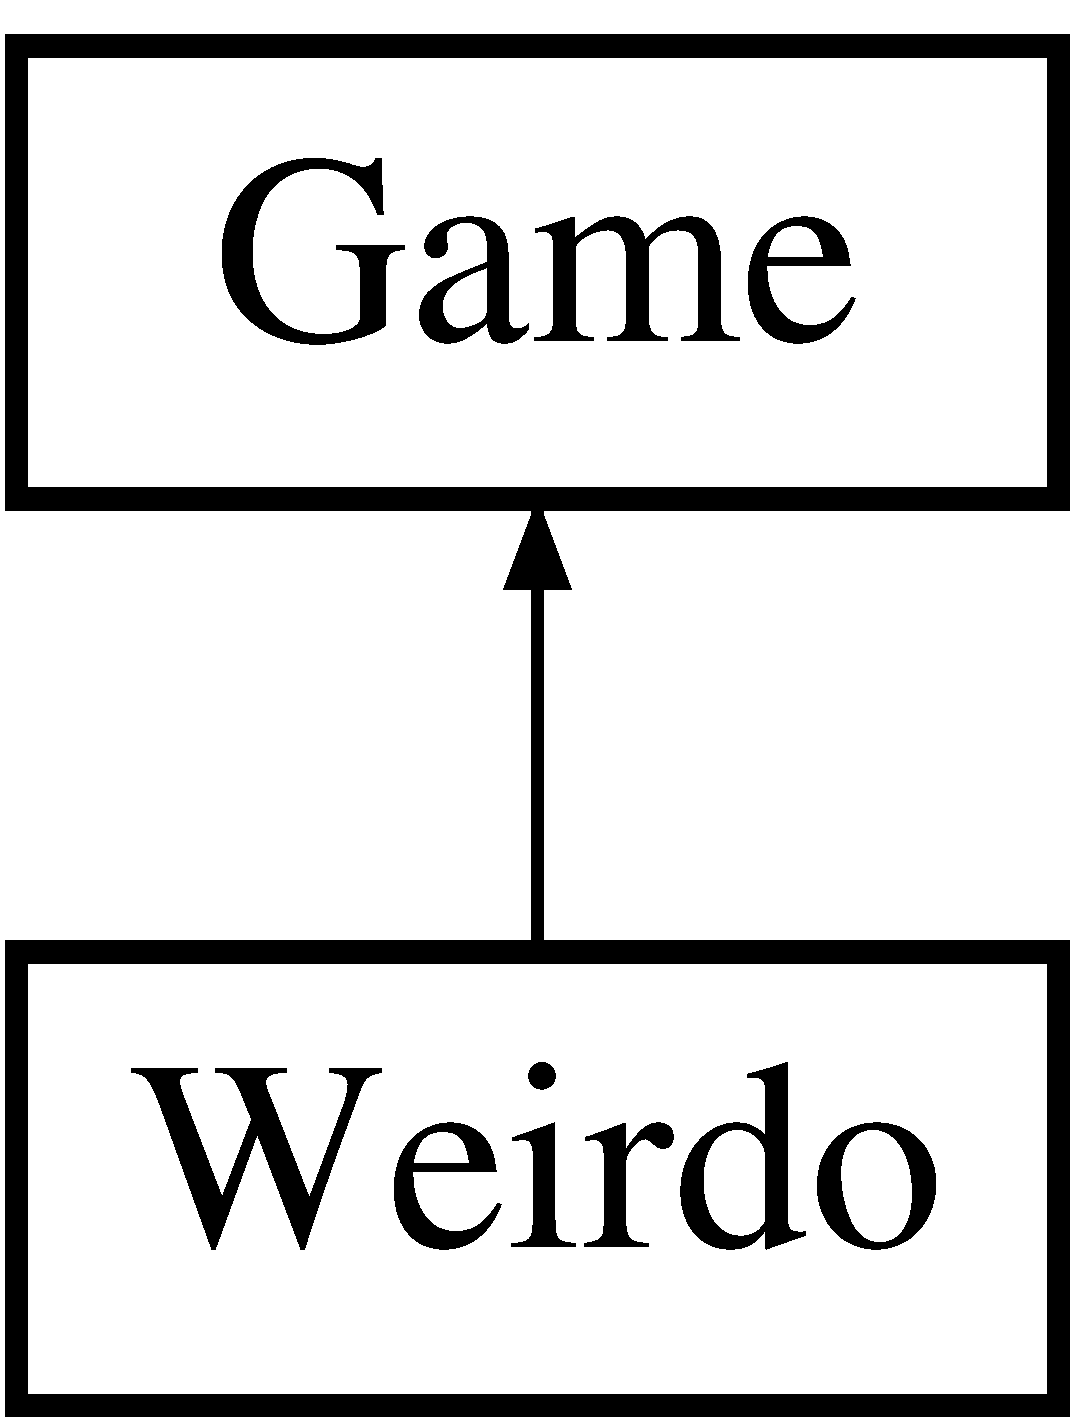
\includegraphics[height=2.000000cm]{class_weirdo}
\end{center}
\end{figure}
\subsection*{Public Member Functions}
\begin{DoxyCompactItemize}
\item 
\hyperlink{class_weirdo_aa4da5eda496d8a5bdfa0bd2e1f4dc582}{Weirdo} ()
\item 
void \hyperlink{class_weirdo_aa71d633becb93a3d1b6273f5b0a8dc14}{set\+Map} (\hyperlink{class_guess}{Guess}, char)
\end{DoxyCompactItemize}
\subsection*{Additional Inherited Members}


\subsection{Detailed Description}


Definition at line 18 of file Weirdo.\+h.



\subsection{Constructor \& Destructor Documentation}
\mbox{\Hypertarget{class_weirdo_aa4da5eda496d8a5bdfa0bd2e1f4dc582}\label{class_weirdo_aa4da5eda496d8a5bdfa0bd2e1f4dc582}} 
\index{Weirdo@{Weirdo}!Weirdo@{Weirdo}}
\index{Weirdo@{Weirdo}!Weirdo@{Weirdo}}
\subsubsection{\texorpdfstring{Weirdo()}{Weirdo()}}
{\footnotesize\ttfamily Weirdo\+::\+Weirdo (\begin{DoxyParamCaption}{ }\end{DoxyParamCaption})\hspace{0.3cm}{\ttfamily [inline]}}



Definition at line 23 of file Weirdo.\+h.



\subsection{Member Function Documentation}
\mbox{\Hypertarget{class_weirdo_aa71d633becb93a3d1b6273f5b0a8dc14}\label{class_weirdo_aa71d633becb93a3d1b6273f5b0a8dc14}} 
\index{Weirdo@{Weirdo}!set\+Map@{set\+Map}}
\index{set\+Map@{set\+Map}!Weirdo@{Weirdo}}
\subsubsection{\texorpdfstring{set\+Map()}{setMap()}}
{\footnotesize\ttfamily void Weirdo\+::set\+Map (\begin{DoxyParamCaption}\item[{\hyperlink{class_guess}{Guess}}]{shot,  }\item[{char}]{dat }\end{DoxyParamCaption})\hspace{0.3cm}{\ttfamily [virtual]}}



Reimplemented from \hyperlink{class_game_a4e23ede628f25d35813322e4e3f46b01}{Game}.



Definition at line 16 of file Weirdo.\+cpp.



The documentation for this class was generated from the following files\+:\begin{DoxyCompactItemize}
\item 
/\+Users/scott\+\_\+r\+\_\+parker/\+Desktop/\+Git\+Hub\+Projects/\+C\+S\+C-\/17\+A-\/42636/\+Project/\+Project2/\+Battle\+Ship\+\_\+\+Project2\+\_\+\+Final\+\_\+\+Version/\hyperlink{_weirdo_8h}{Weirdo.\+h}\item 
/\+Users/scott\+\_\+r\+\_\+parker/\+Desktop/\+Git\+Hub\+Projects/\+C\+S\+C-\/17\+A-\/42636/\+Project/\+Project2/\+Battle\+Ship\+\_\+\+Project2\+\_\+\+Final\+\_\+\+Version/\hyperlink{_weirdo_8cpp}{Weirdo.\+cpp}\end{DoxyCompactItemize}

\chapter{File Documentation}
\hypertarget{_8dep_8inc}{}\section{/\+Users/scott\+\_\+r\+\_\+parker/\+Desktop/\+Git\+Hub\+Projects/\+C\+S\+C-\/17\+A-\/42636/\+Project/\+Project2/\+Battle\+Ship\+\_\+\+Project2\+\_\+\+Final\+\_\+\+Version/.dep.\+inc File Reference}
\label{_8dep_8inc}\index{/\+Users/scott\+\_\+r\+\_\+parker/\+Desktop/\+Git\+Hub\+Projects/\+C\+S\+C-\/17\+A-\/42636/\+Project/\+Project2/\+Battle\+Ship\+\_\+\+Project2\+\_\+\+Final\+\_\+\+Version/.\+dep.\+inc@{/\+Users/scott\+\_\+r\+\_\+parker/\+Desktop/\+Git\+Hub\+Projects/\+C\+S\+C-\/17\+A-\/42636/\+Project/\+Project2/\+Battle\+Ship\+\_\+\+Project2\+\_\+\+Final\+\_\+\+Version/.\+dep.\+inc}}

\hypertarget{_abs_game_8h}{}\section{/\+Users/scott\+\_\+r\+\_\+parker/\+Desktop/\+Git\+Hub\+Projects/\+C\+S\+C-\/17\+A-\/42636/\+Project/\+Project2/\+Battle\+Ship\+\_\+\+Project2\+\_\+\+Final\+\_\+\+Version/\+Abs\+Game.h File Reference}
\label{_abs_game_8h}\index{/\+Users/scott\+\_\+r\+\_\+parker/\+Desktop/\+Git\+Hub\+Projects/\+C\+S\+C-\/17\+A-\/42636/\+Project/\+Project2/\+Battle\+Ship\+\_\+\+Project2\+\_\+\+Final\+\_\+\+Version/\+Abs\+Game.\+h@{/\+Users/scott\+\_\+r\+\_\+parker/\+Desktop/\+Git\+Hub\+Projects/\+C\+S\+C-\/17\+A-\/42636/\+Project/\+Project2/\+Battle\+Ship\+\_\+\+Project2\+\_\+\+Final\+\_\+\+Version/\+Abs\+Game.\+h}}
\subsection*{Classes}
\begin{DoxyCompactItemize}
\item 
class \hyperlink{class_abs_game}{Abs\+Game}
\end{DoxyCompactItemize}

\hypertarget{_game_8o_8d}{}\section{/\+Users/scott\+\_\+r\+\_\+parker/\+Desktop/\+Git\+Hub\+Projects/\+C\+S\+C-\/17\+A-\/42636/\+Project/\+Project2/\+Battle\+Ship\+\_\+\+Project2\+\_\+\+Final\+\_\+\+Version/build/\+Debug/\+G\+N\+U-\/\+Mac\+O\+S\+X/\+Game.o.\+d File Reference}
\label{_game_8o_8d}\index{/\+Users/scott\+\_\+r\+\_\+parker/\+Desktop/\+Git\+Hub\+Projects/\+C\+S\+C-\/17\+A-\/42636/\+Project/\+Project2/\+Battle\+Ship\+\_\+\+Project2\+\_\+\+Final\+\_\+\+Version/build/\+Debug/\+G\+N\+U-\/\+Mac\+O\+S\+X/\+Game.\+o.\+d@{/\+Users/scott\+\_\+r\+\_\+parker/\+Desktop/\+Git\+Hub\+Projects/\+C\+S\+C-\/17\+A-\/42636/\+Project/\+Project2/\+Battle\+Ship\+\_\+\+Project2\+\_\+\+Final\+\_\+\+Version/build/\+Debug/\+G\+N\+U-\/\+Mac\+O\+S\+X/\+Game.\+o.\+d}}

\hypertarget{_guess_8o_8d}{}\section{/\+Users/scott\+\_\+r\+\_\+parker/\+Desktop/\+Git\+Hub\+Projects/\+C\+S\+C-\/17\+A-\/42636/\+Project/\+Project2/\+Battle\+Ship\+\_\+\+Project2\+\_\+\+Final\+\_\+\+Version/build/\+Debug/\+G\+N\+U-\/\+Mac\+O\+S\+X/\+Guess.o.\+d File Reference}
\label{_guess_8o_8d}\index{/\+Users/scott\+\_\+r\+\_\+parker/\+Desktop/\+Git\+Hub\+Projects/\+C\+S\+C-\/17\+A-\/42636/\+Project/\+Project2/\+Battle\+Ship\+\_\+\+Project2\+\_\+\+Final\+\_\+\+Version/build/\+Debug/\+G\+N\+U-\/\+Mac\+O\+S\+X/\+Guess.\+o.\+d@{/\+Users/scott\+\_\+r\+\_\+parker/\+Desktop/\+Git\+Hub\+Projects/\+C\+S\+C-\/17\+A-\/42636/\+Project/\+Project2/\+Battle\+Ship\+\_\+\+Project2\+\_\+\+Final\+\_\+\+Version/build/\+Debug/\+G\+N\+U-\/\+Mac\+O\+S\+X/\+Guess.\+o.\+d}}

\hypertarget{main_8o_8d}{}\section{/\+Users/scott\+\_\+r\+\_\+parker/\+Desktop/\+Git\+Hub\+Projects/\+C\+S\+C-\/17\+A-\/42636/\+Project/\+Project2/\+Battle\+Ship\+\_\+\+Project2\+\_\+\+Final\+\_\+\+Version/build/\+Debug/\+G\+N\+U-\/\+Mac\+O\+S\+X/main.o.\+d File Reference}
\label{main_8o_8d}\index{/\+Users/scott\+\_\+r\+\_\+parker/\+Desktop/\+Git\+Hub\+Projects/\+C\+S\+C-\/17\+A-\/42636/\+Project/\+Project2/\+Battle\+Ship\+\_\+\+Project2\+\_\+\+Final\+\_\+\+Version/build/\+Debug/\+G\+N\+U-\/\+Mac\+O\+S\+X/main.\+o.\+d@{/\+Users/scott\+\_\+r\+\_\+parker/\+Desktop/\+Git\+Hub\+Projects/\+C\+S\+C-\/17\+A-\/42636/\+Project/\+Project2/\+Battle\+Ship\+\_\+\+Project2\+\_\+\+Final\+\_\+\+Version/build/\+Debug/\+G\+N\+U-\/\+Mac\+O\+S\+X/main.\+o.\+d}}

\hypertarget{_weirdo_8o_8d}{}\section{/\+Users/scott\+\_\+r\+\_\+parker/\+Desktop/\+Git\+Hub\+Projects/\+C\+S\+C-\/17\+A-\/42636/\+Project/\+Project2/\+Battle\+Ship\+\_\+\+Project2\+\_\+\+Final\+\_\+\+Version/build/\+Debug/\+G\+N\+U-\/\+Mac\+O\+S\+X/\+Weirdo.o.\+d File Reference}
\label{_weirdo_8o_8d}\index{/\+Users/scott\+\_\+r\+\_\+parker/\+Desktop/\+Git\+Hub\+Projects/\+C\+S\+C-\/17\+A-\/42636/\+Project/\+Project2/\+Battle\+Ship\+\_\+\+Project2\+\_\+\+Final\+\_\+\+Version/build/\+Debug/\+G\+N\+U-\/\+Mac\+O\+S\+X/\+Weirdo.\+o.\+d@{/\+Users/scott\+\_\+r\+\_\+parker/\+Desktop/\+Git\+Hub\+Projects/\+C\+S\+C-\/17\+A-\/42636/\+Project/\+Project2/\+Battle\+Ship\+\_\+\+Project2\+\_\+\+Final\+\_\+\+Version/build/\+Debug/\+G\+N\+U-\/\+Mac\+O\+S\+X/\+Weirdo.\+o.\+d}}

\hypertarget{colors_8h}{}\section{C\+:/\+Users/rcc/\+Desktop/\+C\+S\+C-\/17\+A-\/42636/\+Project/\+Project2/\+Battle\+Ship\+P2\+\_\+\+Final\+Version/colors.h File Reference}
\label{colors_8h}\index{C\+:/\+Users/rcc/\+Desktop/\+C\+S\+C-\/17\+A-\/42636/\+Project/\+Project2/\+Battle\+Ship\+P2\+\_\+\+Final\+Version/colors.\+h@{C\+:/\+Users/rcc/\+Desktop/\+C\+S\+C-\/17\+A-\/42636/\+Project/\+Project2/\+Battle\+Ship\+P2\+\_\+\+Final\+Version/colors.\+h}}
\subsection*{Macros}
\begin{DoxyCompactItemize}
\item 
\#define \hyperlink{colors_8h_ab702106cf3b3e96750b6845ded4e0299}{R\+E\+S\+ET}~\char`\"{}\textbackslash{}033\mbox{[}0m\char`\"{}
\item 
\#define \hyperlink{colors_8h_a7b3b25cba33b07c303f3060fe41887f6}{B\+L\+A\+CK}~\char`\"{}\textbackslash{}033\mbox{[}30m\char`\"{}      /$\ast$ Black $\ast$/
\item 
\#define \hyperlink{colors_8h_a8d23feea868a983c8c2b661e1e16972f}{R\+ED}~\char`\"{}\textbackslash{}033\mbox{[}31m\char`\"{}      /$\ast$ Red $\ast$/
\item 
\#define \hyperlink{colors_8h_acfbc006ea433ad708fdee3e82996e721}{G\+R\+E\+EN}~\char`\"{}\textbackslash{}033\mbox{[}32m\char`\"{}      /$\ast$ Green $\ast$/
\item 
\#define \hyperlink{colors_8h_abf681265909adf3d3e8116c93c0ba179}{Y\+E\+L\+L\+OW}~\char`\"{}\textbackslash{}033\mbox{[}33m\char`\"{}      /$\ast$ Yellow $\ast$/
\item 
\#define \hyperlink{colors_8h_a79d10e672abb49ad63eeaa8aaef57c38}{B\+L\+UE}~\char`\"{}\textbackslash{}033\mbox{[}34m\char`\"{}      /$\ast$ Blue $\ast$/
\item 
\#define \hyperlink{colors_8h_a6f699060902f800f12aaae150f3a708e}{M\+A\+G\+E\+N\+TA}~\char`\"{}\textbackslash{}033\mbox{[}35m\char`\"{}      /$\ast$ Magenta $\ast$/
\item 
\#define \hyperlink{colors_8h_ad243f93c16bc4c1d3e0a13b84421d760}{C\+Y\+AN}~\char`\"{}\textbackslash{}033\mbox{[}36m\char`\"{}      /$\ast$ Cyan $\ast$/
\item 
\#define \hyperlink{colors_8h_a87b537f5fa5c109d3c05c13d6b18f382}{W\+H\+I\+TE}~\char`\"{}\textbackslash{}033\mbox{[}37m\char`\"{}      /$\ast$ White $\ast$/
\item 
\#define \hyperlink{colors_8h_aef2fe95894117165b29036718221979f}{B\+O\+L\+D\+B\+L\+A\+CK}~\char`\"{}\textbackslash{}033\mbox{[}1m\textbackslash{}033\mbox{[}30m\char`\"{}      /$\ast$ Bold Black $\ast$/
\item 
\#define \hyperlink{colors_8h_ab912d02c7998c3d47d05f87be4e2c920}{B\+O\+L\+D\+R\+ED}~\char`\"{}\textbackslash{}033\mbox{[}1m\textbackslash{}033\mbox{[}31m\char`\"{}      /$\ast$ Bold Red $\ast$/
\item 
\#define \hyperlink{colors_8h_a4a6c893a1703c33ede7d702fe5f97c91}{B\+O\+L\+D\+G\+R\+E\+EN}~\char`\"{}\textbackslash{}033\mbox{[}1m\textbackslash{}033\mbox{[}32m\char`\"{}      /$\ast$ Bold Green $\ast$/
\item 
\#define \hyperlink{colors_8h_a8cec79108dfc3c61e8e32d390ec28b26}{B\+O\+L\+D\+Y\+E\+L\+L\+OW}~\char`\"{}\textbackslash{}033\mbox{[}1m\textbackslash{}033\mbox{[}33m\char`\"{}      /$\ast$ Bold Yellow $\ast$/
\item 
\#define \hyperlink{colors_8h_a11e77c19555cbd15bcc744ff36a18635}{B\+O\+L\+D\+B\+L\+UE}~\char`\"{}\textbackslash{}033\mbox{[}1m\textbackslash{}033\mbox{[}34m\char`\"{}      /$\ast$ Bold Blue $\ast$/
\item 
\#define \hyperlink{colors_8h_ac4723c5ee12cfca16e2172b57b99cb07}{B\+O\+L\+D\+M\+A\+G\+E\+N\+TA}~\char`\"{}\textbackslash{}033\mbox{[}1m\textbackslash{}033\mbox{[}35m\char`\"{}      /$\ast$ Bold Magenta $\ast$/
\item 
\#define \hyperlink{colors_8h_ae87af5e6363eb1913b17f24dcb60a22d}{B\+O\+L\+D\+C\+Y\+AN}~\char`\"{}\textbackslash{}033\mbox{[}1m\textbackslash{}033\mbox{[}36m\char`\"{}      /$\ast$ Bold Cyan $\ast$/
\item 
\#define \hyperlink{colors_8h_aa4ef051614aa0bd503b0a18ee158c5d7}{B\+O\+L\+D\+W\+H\+I\+TE}~\char`\"{}\textbackslash{}033\mbox{[}1m\textbackslash{}033\mbox{[}37m\char`\"{}      /$\ast$ Bold White $\ast$/
\item 
\#define \hyperlink{colors_8h_ade269cc47cfaba70068f2586e898051d}{I\+N\+V\+E\+R\+SE}~\char`\"{}\textbackslash{}033\mbox{[}7m\char`\"{}     /$\ast$ Swap Bacground and Text colors $\ast$/
\item 
\#define \hyperlink{colors_8h_aaec1a65734e33bc49e8dc8d90e9546bc}{U\+N\+D\+E\+R\+L\+I\+NE}~\char`\"{}\textbackslash{}033\mbox{[}4m\char`\"{}     /$\ast$ Underline Single $\ast$/
\item 
\#define \hyperlink{colors_8h_ab4724fec8e2574110f93d0cebf25ac92}{B\+G\+B\+L\+A\+CK}~\char`\"{}\textbackslash{}033\mbox{[}40m\char`\"{}      /$\ast$ B\+L\+A\+C\+K Background $\ast$/
\item 
\#define \hyperlink{colors_8h_a95e0a3871c4ee628ff78494e0c4e459a}{B\+G\+R\+ED}~\char`\"{}\textbackslash{}033\mbox{[}41m\char`\"{}      /$\ast$ R\+E\+D Background $\ast$/
\item 
\#define \hyperlink{colors_8h_a898cbb3b8ecef2510cb6152b1f96d4c8}{B\+G\+G\+R\+E\+EN}~\char`\"{}\textbackslash{}033\mbox{[}42m\char`\"{}      /$\ast$ G\+R\+E\+E\+N Background $\ast$/
\item 
\#define \hyperlink{colors_8h_ab68b1d2fc1f910b83d749ffa0a9a37f8}{B\+G\+Y\+E\+L\+L\+OW}~\char`\"{}\textbackslash{}033\mbox{[}43m\char`\"{}      /$\ast$ Y\+E\+L\+L\+O\+W Background $\ast$/
\item 
\#define \hyperlink{colors_8h_a2c546b464622d186d669cfd8a4fa2947}{B\+G\+B\+L\+UE}~\char`\"{}\textbackslash{}033\mbox{[}44m\char`\"{}      /$\ast$ B\+L\+U\+E Background $\ast$/
\item 
\#define \hyperlink{colors_8h_a96a8e22829e03241b315f0e8b34b49ad}{B\+G\+M\+A\+G\+E\+N\+TA}~\char`\"{}\textbackslash{}033\mbox{[}45m\char`\"{}      /$\ast$ M\+A\+G\+E\+N\+T\+A Background $\ast$/
\item 
\#define \hyperlink{colors_8h_ade07cf7b38b0c36751e9c9880cb8792c}{B\+G\+C\+Y\+AN}~\char`\"{}\textbackslash{}033\mbox{[}46m\char`\"{}      /$\ast$ C\+Y\+A\+N Background $\ast$/
\item 
\#define \hyperlink{colors_8h_ac7aa010e8e3ad6bbf4c725e52ba02168}{B\+G\+W\+H\+I\+TE}~\char`\"{}\textbackslash{}033\mbox{[}47m\char`\"{}      /$\ast$ W\+H\+I\+T\+E Background $\ast$/
\end{DoxyCompactItemize}


\subsection{Macro Definition Documentation}
\index{colors.\+h@{colors.\+h}!B\+G\+B\+L\+A\+CK@{B\+G\+B\+L\+A\+CK}}
\index{B\+G\+B\+L\+A\+CK@{B\+G\+B\+L\+A\+CK}!colors.\+h@{colors.\+h}}
\subsubsection[{\texorpdfstring{B\+G\+B\+L\+A\+CK}{BGBLACK}}]{\setlength{\rightskip}{0pt plus 5cm}\#define B\+G\+B\+L\+A\+CK~\char`\"{}\textbackslash{}033\mbox{[}40m\char`\"{}      /$\ast$ B\+L\+A\+C\+K Background $\ast$/}\hypertarget{colors_8h_ab4724fec8e2574110f93d0cebf25ac92}{}\label{colors_8h_ab4724fec8e2574110f93d0cebf25ac92}


Definition at line 39 of file colors.\+h.

\index{colors.\+h@{colors.\+h}!B\+G\+B\+L\+UE@{B\+G\+B\+L\+UE}}
\index{B\+G\+B\+L\+UE@{B\+G\+B\+L\+UE}!colors.\+h@{colors.\+h}}
\subsubsection[{\texorpdfstring{B\+G\+B\+L\+UE}{BGBLUE}}]{\setlength{\rightskip}{0pt plus 5cm}\#define B\+G\+B\+L\+UE~\char`\"{}\textbackslash{}033\mbox{[}44m\char`\"{}      /$\ast$ B\+L\+U\+E Background $\ast$/}\hypertarget{colors_8h_a2c546b464622d186d669cfd8a4fa2947}{}\label{colors_8h_a2c546b464622d186d669cfd8a4fa2947}


Definition at line 43 of file colors.\+h.

\index{colors.\+h@{colors.\+h}!B\+G\+C\+Y\+AN@{B\+G\+C\+Y\+AN}}
\index{B\+G\+C\+Y\+AN@{B\+G\+C\+Y\+AN}!colors.\+h@{colors.\+h}}
\subsubsection[{\texorpdfstring{B\+G\+C\+Y\+AN}{BGCYAN}}]{\setlength{\rightskip}{0pt plus 5cm}\#define B\+G\+C\+Y\+AN~\char`\"{}\textbackslash{}033\mbox{[}46m\char`\"{}      /$\ast$ C\+Y\+A\+N Background $\ast$/}\hypertarget{colors_8h_ade07cf7b38b0c36751e9c9880cb8792c}{}\label{colors_8h_ade07cf7b38b0c36751e9c9880cb8792c}


Definition at line 45 of file colors.\+h.

\index{colors.\+h@{colors.\+h}!B\+G\+G\+R\+E\+EN@{B\+G\+G\+R\+E\+EN}}
\index{B\+G\+G\+R\+E\+EN@{B\+G\+G\+R\+E\+EN}!colors.\+h@{colors.\+h}}
\subsubsection[{\texorpdfstring{B\+G\+G\+R\+E\+EN}{BGGREEN}}]{\setlength{\rightskip}{0pt plus 5cm}\#define B\+G\+G\+R\+E\+EN~\char`\"{}\textbackslash{}033\mbox{[}42m\char`\"{}      /$\ast$ G\+R\+E\+E\+N Background $\ast$/}\hypertarget{colors_8h_a898cbb3b8ecef2510cb6152b1f96d4c8}{}\label{colors_8h_a898cbb3b8ecef2510cb6152b1f96d4c8}


Definition at line 41 of file colors.\+h.

\index{colors.\+h@{colors.\+h}!B\+G\+M\+A\+G\+E\+N\+TA@{B\+G\+M\+A\+G\+E\+N\+TA}}
\index{B\+G\+M\+A\+G\+E\+N\+TA@{B\+G\+M\+A\+G\+E\+N\+TA}!colors.\+h@{colors.\+h}}
\subsubsection[{\texorpdfstring{B\+G\+M\+A\+G\+E\+N\+TA}{BGMAGENTA}}]{\setlength{\rightskip}{0pt plus 5cm}\#define B\+G\+M\+A\+G\+E\+N\+TA~\char`\"{}\textbackslash{}033\mbox{[}45m\char`\"{}      /$\ast$ M\+A\+G\+E\+N\+T\+A Background $\ast$/}\hypertarget{colors_8h_a96a8e22829e03241b315f0e8b34b49ad}{}\label{colors_8h_a96a8e22829e03241b315f0e8b34b49ad}


Definition at line 44 of file colors.\+h.

\index{colors.\+h@{colors.\+h}!B\+G\+R\+ED@{B\+G\+R\+ED}}
\index{B\+G\+R\+ED@{B\+G\+R\+ED}!colors.\+h@{colors.\+h}}
\subsubsection[{\texorpdfstring{B\+G\+R\+ED}{BGRED}}]{\setlength{\rightskip}{0pt plus 5cm}\#define B\+G\+R\+ED~\char`\"{}\textbackslash{}033\mbox{[}41m\char`\"{}      /$\ast$ R\+E\+D Background $\ast$/}\hypertarget{colors_8h_a95e0a3871c4ee628ff78494e0c4e459a}{}\label{colors_8h_a95e0a3871c4ee628ff78494e0c4e459a}


Definition at line 40 of file colors.\+h.

\index{colors.\+h@{colors.\+h}!B\+G\+W\+H\+I\+TE@{B\+G\+W\+H\+I\+TE}}
\index{B\+G\+W\+H\+I\+TE@{B\+G\+W\+H\+I\+TE}!colors.\+h@{colors.\+h}}
\subsubsection[{\texorpdfstring{B\+G\+W\+H\+I\+TE}{BGWHITE}}]{\setlength{\rightskip}{0pt plus 5cm}\#define B\+G\+W\+H\+I\+TE~\char`\"{}\textbackslash{}033\mbox{[}47m\char`\"{}      /$\ast$ W\+H\+I\+T\+E Background $\ast$/}\hypertarget{colors_8h_ac7aa010e8e3ad6bbf4c725e52ba02168}{}\label{colors_8h_ac7aa010e8e3ad6bbf4c725e52ba02168}


Definition at line 46 of file colors.\+h.

\index{colors.\+h@{colors.\+h}!B\+G\+Y\+E\+L\+L\+OW@{B\+G\+Y\+E\+L\+L\+OW}}
\index{B\+G\+Y\+E\+L\+L\+OW@{B\+G\+Y\+E\+L\+L\+OW}!colors.\+h@{colors.\+h}}
\subsubsection[{\texorpdfstring{B\+G\+Y\+E\+L\+L\+OW}{BGYELLOW}}]{\setlength{\rightskip}{0pt plus 5cm}\#define B\+G\+Y\+E\+L\+L\+OW~\char`\"{}\textbackslash{}033\mbox{[}43m\char`\"{}      /$\ast$ Y\+E\+L\+L\+O\+W Background $\ast$/}\hypertarget{colors_8h_ab68b1d2fc1f910b83d749ffa0a9a37f8}{}\label{colors_8h_ab68b1d2fc1f910b83d749ffa0a9a37f8}


Definition at line 42 of file colors.\+h.

\index{colors.\+h@{colors.\+h}!B\+L\+A\+CK@{B\+L\+A\+CK}}
\index{B\+L\+A\+CK@{B\+L\+A\+CK}!colors.\+h@{colors.\+h}}
\subsubsection[{\texorpdfstring{B\+L\+A\+CK}{BLACK}}]{\setlength{\rightskip}{0pt plus 5cm}\#define B\+L\+A\+CK~\char`\"{}\textbackslash{}033\mbox{[}30m\char`\"{}      /$\ast$ Black $\ast$/}\hypertarget{colors_8h_a7b3b25cba33b07c303f3060fe41887f6}{}\label{colors_8h_a7b3b25cba33b07c303f3060fe41887f6}


Definition at line 19 of file colors.\+h.

\index{colors.\+h@{colors.\+h}!B\+L\+UE@{B\+L\+UE}}
\index{B\+L\+UE@{B\+L\+UE}!colors.\+h@{colors.\+h}}
\subsubsection[{\texorpdfstring{B\+L\+UE}{BLUE}}]{\setlength{\rightskip}{0pt plus 5cm}\#define B\+L\+UE~\char`\"{}\textbackslash{}033\mbox{[}34m\char`\"{}      /$\ast$ Blue $\ast$/}\hypertarget{colors_8h_a79d10e672abb49ad63eeaa8aaef57c38}{}\label{colors_8h_a79d10e672abb49ad63eeaa8aaef57c38}


Definition at line 23 of file colors.\+h.

\index{colors.\+h@{colors.\+h}!B\+O\+L\+D\+B\+L\+A\+CK@{B\+O\+L\+D\+B\+L\+A\+CK}}
\index{B\+O\+L\+D\+B\+L\+A\+CK@{B\+O\+L\+D\+B\+L\+A\+CK}!colors.\+h@{colors.\+h}}
\subsubsection[{\texorpdfstring{B\+O\+L\+D\+B\+L\+A\+CK}{BOLDBLACK}}]{\setlength{\rightskip}{0pt plus 5cm}\#define B\+O\+L\+D\+B\+L\+A\+CK~\char`\"{}\textbackslash{}033\mbox{[}1m\textbackslash{}033\mbox{[}30m\char`\"{}      /$\ast$ Bold Black $\ast$/}\hypertarget{colors_8h_aef2fe95894117165b29036718221979f}{}\label{colors_8h_aef2fe95894117165b29036718221979f}


Definition at line 27 of file colors.\+h.

\index{colors.\+h@{colors.\+h}!B\+O\+L\+D\+B\+L\+UE@{B\+O\+L\+D\+B\+L\+UE}}
\index{B\+O\+L\+D\+B\+L\+UE@{B\+O\+L\+D\+B\+L\+UE}!colors.\+h@{colors.\+h}}
\subsubsection[{\texorpdfstring{B\+O\+L\+D\+B\+L\+UE}{BOLDBLUE}}]{\setlength{\rightskip}{0pt plus 5cm}\#define B\+O\+L\+D\+B\+L\+UE~\char`\"{}\textbackslash{}033\mbox{[}1m\textbackslash{}033\mbox{[}34m\char`\"{}      /$\ast$ Bold Blue $\ast$/}\hypertarget{colors_8h_a11e77c19555cbd15bcc744ff36a18635}{}\label{colors_8h_a11e77c19555cbd15bcc744ff36a18635}


Definition at line 31 of file colors.\+h.

\index{colors.\+h@{colors.\+h}!B\+O\+L\+D\+C\+Y\+AN@{B\+O\+L\+D\+C\+Y\+AN}}
\index{B\+O\+L\+D\+C\+Y\+AN@{B\+O\+L\+D\+C\+Y\+AN}!colors.\+h@{colors.\+h}}
\subsubsection[{\texorpdfstring{B\+O\+L\+D\+C\+Y\+AN}{BOLDCYAN}}]{\setlength{\rightskip}{0pt plus 5cm}\#define B\+O\+L\+D\+C\+Y\+AN~\char`\"{}\textbackslash{}033\mbox{[}1m\textbackslash{}033\mbox{[}36m\char`\"{}      /$\ast$ Bold Cyan $\ast$/}\hypertarget{colors_8h_ae87af5e6363eb1913b17f24dcb60a22d}{}\label{colors_8h_ae87af5e6363eb1913b17f24dcb60a22d}


Definition at line 33 of file colors.\+h.

\index{colors.\+h@{colors.\+h}!B\+O\+L\+D\+G\+R\+E\+EN@{B\+O\+L\+D\+G\+R\+E\+EN}}
\index{B\+O\+L\+D\+G\+R\+E\+EN@{B\+O\+L\+D\+G\+R\+E\+EN}!colors.\+h@{colors.\+h}}
\subsubsection[{\texorpdfstring{B\+O\+L\+D\+G\+R\+E\+EN}{BOLDGREEN}}]{\setlength{\rightskip}{0pt plus 5cm}\#define B\+O\+L\+D\+G\+R\+E\+EN~\char`\"{}\textbackslash{}033\mbox{[}1m\textbackslash{}033\mbox{[}32m\char`\"{}      /$\ast$ Bold Green $\ast$/}\hypertarget{colors_8h_a4a6c893a1703c33ede7d702fe5f97c91}{}\label{colors_8h_a4a6c893a1703c33ede7d702fe5f97c91}


Definition at line 29 of file colors.\+h.

\index{colors.\+h@{colors.\+h}!B\+O\+L\+D\+M\+A\+G\+E\+N\+TA@{B\+O\+L\+D\+M\+A\+G\+E\+N\+TA}}
\index{B\+O\+L\+D\+M\+A\+G\+E\+N\+TA@{B\+O\+L\+D\+M\+A\+G\+E\+N\+TA}!colors.\+h@{colors.\+h}}
\subsubsection[{\texorpdfstring{B\+O\+L\+D\+M\+A\+G\+E\+N\+TA}{BOLDMAGENTA}}]{\setlength{\rightskip}{0pt plus 5cm}\#define B\+O\+L\+D\+M\+A\+G\+E\+N\+TA~\char`\"{}\textbackslash{}033\mbox{[}1m\textbackslash{}033\mbox{[}35m\char`\"{}      /$\ast$ Bold Magenta $\ast$/}\hypertarget{colors_8h_ac4723c5ee12cfca16e2172b57b99cb07}{}\label{colors_8h_ac4723c5ee12cfca16e2172b57b99cb07}


Definition at line 32 of file colors.\+h.

\index{colors.\+h@{colors.\+h}!B\+O\+L\+D\+R\+ED@{B\+O\+L\+D\+R\+ED}}
\index{B\+O\+L\+D\+R\+ED@{B\+O\+L\+D\+R\+ED}!colors.\+h@{colors.\+h}}
\subsubsection[{\texorpdfstring{B\+O\+L\+D\+R\+ED}{BOLDRED}}]{\setlength{\rightskip}{0pt plus 5cm}\#define B\+O\+L\+D\+R\+ED~\char`\"{}\textbackslash{}033\mbox{[}1m\textbackslash{}033\mbox{[}31m\char`\"{}      /$\ast$ Bold Red $\ast$/}\hypertarget{colors_8h_ab912d02c7998c3d47d05f87be4e2c920}{}\label{colors_8h_ab912d02c7998c3d47d05f87be4e2c920}


Definition at line 28 of file colors.\+h.

\index{colors.\+h@{colors.\+h}!B\+O\+L\+D\+W\+H\+I\+TE@{B\+O\+L\+D\+W\+H\+I\+TE}}
\index{B\+O\+L\+D\+W\+H\+I\+TE@{B\+O\+L\+D\+W\+H\+I\+TE}!colors.\+h@{colors.\+h}}
\subsubsection[{\texorpdfstring{B\+O\+L\+D\+W\+H\+I\+TE}{BOLDWHITE}}]{\setlength{\rightskip}{0pt plus 5cm}\#define B\+O\+L\+D\+W\+H\+I\+TE~\char`\"{}\textbackslash{}033\mbox{[}1m\textbackslash{}033\mbox{[}37m\char`\"{}      /$\ast$ Bold White $\ast$/}\hypertarget{colors_8h_aa4ef051614aa0bd503b0a18ee158c5d7}{}\label{colors_8h_aa4ef051614aa0bd503b0a18ee158c5d7}


Definition at line 34 of file colors.\+h.

\index{colors.\+h@{colors.\+h}!B\+O\+L\+D\+Y\+E\+L\+L\+OW@{B\+O\+L\+D\+Y\+E\+L\+L\+OW}}
\index{B\+O\+L\+D\+Y\+E\+L\+L\+OW@{B\+O\+L\+D\+Y\+E\+L\+L\+OW}!colors.\+h@{colors.\+h}}
\subsubsection[{\texorpdfstring{B\+O\+L\+D\+Y\+E\+L\+L\+OW}{BOLDYELLOW}}]{\setlength{\rightskip}{0pt plus 5cm}\#define B\+O\+L\+D\+Y\+E\+L\+L\+OW~\char`\"{}\textbackslash{}033\mbox{[}1m\textbackslash{}033\mbox{[}33m\char`\"{}      /$\ast$ Bold Yellow $\ast$/}\hypertarget{colors_8h_a8cec79108dfc3c61e8e32d390ec28b26}{}\label{colors_8h_a8cec79108dfc3c61e8e32d390ec28b26}


Definition at line 30 of file colors.\+h.

\index{colors.\+h@{colors.\+h}!C\+Y\+AN@{C\+Y\+AN}}
\index{C\+Y\+AN@{C\+Y\+AN}!colors.\+h@{colors.\+h}}
\subsubsection[{\texorpdfstring{C\+Y\+AN}{CYAN}}]{\setlength{\rightskip}{0pt plus 5cm}\#define C\+Y\+AN~\char`\"{}\textbackslash{}033\mbox{[}36m\char`\"{}      /$\ast$ Cyan $\ast$/}\hypertarget{colors_8h_ad243f93c16bc4c1d3e0a13b84421d760}{}\label{colors_8h_ad243f93c16bc4c1d3e0a13b84421d760}


Definition at line 25 of file colors.\+h.

\index{colors.\+h@{colors.\+h}!G\+R\+E\+EN@{G\+R\+E\+EN}}
\index{G\+R\+E\+EN@{G\+R\+E\+EN}!colors.\+h@{colors.\+h}}
\subsubsection[{\texorpdfstring{G\+R\+E\+EN}{GREEN}}]{\setlength{\rightskip}{0pt plus 5cm}\#define G\+R\+E\+EN~\char`\"{}\textbackslash{}033\mbox{[}32m\char`\"{}      /$\ast$ Green $\ast$/}\hypertarget{colors_8h_acfbc006ea433ad708fdee3e82996e721}{}\label{colors_8h_acfbc006ea433ad708fdee3e82996e721}


Definition at line 21 of file colors.\+h.

\index{colors.\+h@{colors.\+h}!I\+N\+V\+E\+R\+SE@{I\+N\+V\+E\+R\+SE}}
\index{I\+N\+V\+E\+R\+SE@{I\+N\+V\+E\+R\+SE}!colors.\+h@{colors.\+h}}
\subsubsection[{\texorpdfstring{I\+N\+V\+E\+R\+SE}{INVERSE}}]{\setlength{\rightskip}{0pt plus 5cm}\#define I\+N\+V\+E\+R\+SE~\char`\"{}\textbackslash{}033\mbox{[}7m\char`\"{}     /$\ast$ Swap Bacground and Text colors $\ast$/}\hypertarget{colors_8h_ade269cc47cfaba70068f2586e898051d}{}\label{colors_8h_ade269cc47cfaba70068f2586e898051d}


Definition at line 36 of file colors.\+h.

\index{colors.\+h@{colors.\+h}!M\+A\+G\+E\+N\+TA@{M\+A\+G\+E\+N\+TA}}
\index{M\+A\+G\+E\+N\+TA@{M\+A\+G\+E\+N\+TA}!colors.\+h@{colors.\+h}}
\subsubsection[{\texorpdfstring{M\+A\+G\+E\+N\+TA}{MAGENTA}}]{\setlength{\rightskip}{0pt plus 5cm}\#define M\+A\+G\+E\+N\+TA~\char`\"{}\textbackslash{}033\mbox{[}35m\char`\"{}      /$\ast$ Magenta $\ast$/}\hypertarget{colors_8h_a6f699060902f800f12aaae150f3a708e}{}\label{colors_8h_a6f699060902f800f12aaae150f3a708e}


Definition at line 24 of file colors.\+h.

\index{colors.\+h@{colors.\+h}!R\+ED@{R\+ED}}
\index{R\+ED@{R\+ED}!colors.\+h@{colors.\+h}}
\subsubsection[{\texorpdfstring{R\+ED}{RED}}]{\setlength{\rightskip}{0pt plus 5cm}\#define R\+ED~\char`\"{}\textbackslash{}033\mbox{[}31m\char`\"{}      /$\ast$ Red $\ast$/}\hypertarget{colors_8h_a8d23feea868a983c8c2b661e1e16972f}{}\label{colors_8h_a8d23feea868a983c8c2b661e1e16972f}


Definition at line 20 of file colors.\+h.

\index{colors.\+h@{colors.\+h}!R\+E\+S\+ET@{R\+E\+S\+ET}}
\index{R\+E\+S\+ET@{R\+E\+S\+ET}!colors.\+h@{colors.\+h}}
\subsubsection[{\texorpdfstring{R\+E\+S\+ET}{RESET}}]{\setlength{\rightskip}{0pt plus 5cm}\#define R\+E\+S\+ET~\char`\"{}\textbackslash{}033\mbox{[}0m\char`\"{}}\hypertarget{colors_8h_ab702106cf3b3e96750b6845ded4e0299}{}\label{colors_8h_ab702106cf3b3e96750b6845ded4e0299}


Definition at line 18 of file colors.\+h.

\index{colors.\+h@{colors.\+h}!U\+N\+D\+E\+R\+L\+I\+NE@{U\+N\+D\+E\+R\+L\+I\+NE}}
\index{U\+N\+D\+E\+R\+L\+I\+NE@{U\+N\+D\+E\+R\+L\+I\+NE}!colors.\+h@{colors.\+h}}
\subsubsection[{\texorpdfstring{U\+N\+D\+E\+R\+L\+I\+NE}{UNDERLINE}}]{\setlength{\rightskip}{0pt plus 5cm}\#define U\+N\+D\+E\+R\+L\+I\+NE~\char`\"{}\textbackslash{}033\mbox{[}4m\char`\"{}     /$\ast$ Underline Single $\ast$/}\hypertarget{colors_8h_aaec1a65734e33bc49e8dc8d90e9546bc}{}\label{colors_8h_aaec1a65734e33bc49e8dc8d90e9546bc}


Definition at line 37 of file colors.\+h.

\index{colors.\+h@{colors.\+h}!W\+H\+I\+TE@{W\+H\+I\+TE}}
\index{W\+H\+I\+TE@{W\+H\+I\+TE}!colors.\+h@{colors.\+h}}
\subsubsection[{\texorpdfstring{W\+H\+I\+TE}{WHITE}}]{\setlength{\rightskip}{0pt plus 5cm}\#define W\+H\+I\+TE~\char`\"{}\textbackslash{}033\mbox{[}37m\char`\"{}      /$\ast$ White $\ast$/}\hypertarget{colors_8h_a87b537f5fa5c109d3c05c13d6b18f382}{}\label{colors_8h_a87b537f5fa5c109d3c05c13d6b18f382}


Definition at line 26 of file colors.\+h.

\index{colors.\+h@{colors.\+h}!Y\+E\+L\+L\+OW@{Y\+E\+L\+L\+OW}}
\index{Y\+E\+L\+L\+OW@{Y\+E\+L\+L\+OW}!colors.\+h@{colors.\+h}}
\subsubsection[{\texorpdfstring{Y\+E\+L\+L\+OW}{YELLOW}}]{\setlength{\rightskip}{0pt plus 5cm}\#define Y\+E\+L\+L\+OW~\char`\"{}\textbackslash{}033\mbox{[}33m\char`\"{}      /$\ast$ Yellow $\ast$/}\hypertarget{colors_8h_abf681265909adf3d3e8116c93c0ba179}{}\label{colors_8h_abf681265909adf3d3e8116c93c0ba179}


Definition at line 22 of file colors.\+h.


\hypertarget{_game_8cpp}{}\section{/\+Users/scott\+\_\+r\+\_\+parker/\+Desktop/\+Git\+Hub\+Projects/\+C\+S\+C-\/17\+A-\/42636/\+Project/\+Project2/\+Battle\+Ship\+\_\+\+Project2\+\_\+\+Final\+\_\+\+Version/\+Game.cpp File Reference}
\label{_game_8cpp}\index{/\+Users/scott\+\_\+r\+\_\+parker/\+Desktop/\+Git\+Hub\+Projects/\+C\+S\+C-\/17\+A-\/42636/\+Project/\+Project2/\+Battle\+Ship\+\_\+\+Project2\+\_\+\+Final\+\_\+\+Version/\+Game.\+cpp@{/\+Users/scott\+\_\+r\+\_\+parker/\+Desktop/\+Git\+Hub\+Projects/\+C\+S\+C-\/17\+A-\/42636/\+Project/\+Project2/\+Battle\+Ship\+\_\+\+Project2\+\_\+\+Final\+\_\+\+Version/\+Game.\+cpp}}
{\ttfamily \#include \char`\"{}Game.\+h\char`\"{}}\newline
{\ttfamily \#include \char`\"{}colors.\+h\char`\"{}}\newline
\subsection*{Functions}
\begin{DoxyCompactItemize}
\item 
ostream \& \hyperlink{_game_8cpp_adb86a43ea400e0695e0b1ae92dd7a685}{operator$<$$<$} (ostream \&strm, const \hyperlink{class_game}{Game} \&obj)
\end{DoxyCompactItemize}


\subsection{Function Documentation}
\mbox{\Hypertarget{_game_8cpp_adb86a43ea400e0695e0b1ae92dd7a685}\label{_game_8cpp_adb86a43ea400e0695e0b1ae92dd7a685}} 
\index{Game.\+cpp@{Game.\+cpp}!operator$<$$<$@{operator$<$$<$}}
\index{operator$<$$<$@{operator$<$$<$}!Game.\+cpp@{Game.\+cpp}}
\subsubsection{\texorpdfstring{operator$<$$<$()}{operator<<()}}
{\footnotesize\ttfamily ostream\& operator$<$$<$ (\begin{DoxyParamCaption}\item[{ostream \&}]{strm,  }\item[{const \hyperlink{class_game}{Game} \&}]{obj }\end{DoxyParamCaption})}



Definition at line 130 of file Game.\+cpp.


\hypertarget{_game_8h}{}\section{/\+Users/scott\+\_\+r\+\_\+parker/\+Desktop/\+Git\+Hub\+Projects/\+C\+S\+C-\/17\+A-\/42636/\+Project/\+Project2/\+Battle\+Ship\+\_\+\+Project2\+\_\+\+Final\+\_\+\+Version/\+Game.h File Reference}
\label{_game_8h}\index{/\+Users/scott\+\_\+r\+\_\+parker/\+Desktop/\+Git\+Hub\+Projects/\+C\+S\+C-\/17\+A-\/42636/\+Project/\+Project2/\+Battle\+Ship\+\_\+\+Project2\+\_\+\+Final\+\_\+\+Version/\+Game.\+h@{/\+Users/scott\+\_\+r\+\_\+parker/\+Desktop/\+Git\+Hub\+Projects/\+C\+S\+C-\/17\+A-\/42636/\+Project/\+Project2/\+Battle\+Ship\+\_\+\+Project2\+\_\+\+Final\+\_\+\+Version/\+Game.\+h}}
{\ttfamily \#include \char`\"{}Abs\+Game.\+h\char`\"{}}\newline
{\ttfamily \#include \char`\"{}Map.\+h\char`\"{}}\newline
{\ttfamily \#include \char`\"{}Guess.\+h\char`\"{}}\newline
\subsection*{Classes}
\begin{DoxyCompactItemize}
\item 
class \hyperlink{class_game}{Game}
\end{DoxyCompactItemize}
\subsection*{Functions}
\begin{DoxyCompactItemize}
\item 
ostream \& \hyperlink{_game_8h_a7bb9176e07b6f6c73c930dba6400265f}{operator$<$$<$} (ostream \&, const \hyperlink{class_game}{Game} \&)
\end{DoxyCompactItemize}


\subsection{Function Documentation}
\mbox{\Hypertarget{_game_8h_a7bb9176e07b6f6c73c930dba6400265f}\label{_game_8h_a7bb9176e07b6f6c73c930dba6400265f}} 
\index{Game.\+h@{Game.\+h}!operator$<$$<$@{operator$<$$<$}}
\index{operator$<$$<$@{operator$<$$<$}!Game.\+h@{Game.\+h}}
\subsubsection{\texorpdfstring{operator$<$$<$()}{operator<<()}}
{\footnotesize\ttfamily ostream\& operator$<$$<$ (\begin{DoxyParamCaption}\item[{ostream \&}]{,  }\item[{const \hyperlink{class_game}{Game} \&}]{ }\end{DoxyParamCaption})}



Definition at line 130 of file Game.\+cpp.


\hypertarget{_guess_8cpp}{}\section{C\+:/\+Users/rcc/\+Desktop/\+C\+S\+C-\/17\+A-\/42636/\+Project/\+Project2/\+Battle\+Ship\+P2\+\_\+\+Final\+Version/\+Guess.cpp File Reference}
\label{_guess_8cpp}\index{C\+:/\+Users/rcc/\+Desktop/\+C\+S\+C-\/17\+A-\/42636/\+Project/\+Project2/\+Battle\+Ship\+P2\+\_\+\+Final\+Version/\+Guess.\+cpp@{C\+:/\+Users/rcc/\+Desktop/\+C\+S\+C-\/17\+A-\/42636/\+Project/\+Project2/\+Battle\+Ship\+P2\+\_\+\+Final\+Version/\+Guess.\+cpp}}
{\ttfamily \#include $<$cctype$>$}\\*
{\ttfamily \#include \char`\"{}Guess.\+h\char`\"{}}\\*
\subsection*{Functions}
\begin{DoxyCompactItemize}
\item 
ostream \& \hyperlink{_guess_8cpp_a10577937ad464953e1a72c644b1f55ea}{operator$<$$<$} (ostream \&strm, const \hyperlink{class_guess}{Guess} \&obj)
\item 
istream \& \hyperlink{_guess_8cpp_a03e0c5f22ff50d7d7affd025624d9648}{operator$>$$>$} (istream \&strm, \hyperlink{class_guess}{Guess} \&obj)
\end{DoxyCompactItemize}


\subsection{Function Documentation}
\index{Guess.\+cpp@{Guess.\+cpp}!operator$<$$<$@{operator$<$$<$}}
\index{operator$<$$<$@{operator$<$$<$}!Guess.\+cpp@{Guess.\+cpp}}
\subsubsection[{\texorpdfstring{operator$<$$<$(ostream \&strm, const Guess \&obj)}{operator<<(ostream &strm, const Guess &obj)}}]{\setlength{\rightskip}{0pt plus 5cm}ostream\& operator$<$$<$ (
\begin{DoxyParamCaption}
\item[{ostream \&}]{strm, }
\item[{const {\bf Guess} \&}]{obj}
\end{DoxyParamCaption}
)}\hypertarget{_guess_8cpp_a10577937ad464953e1a72c644b1f55ea}{}\label{_guess_8cpp_a10577937ad464953e1a72c644b1f55ea}


Definition at line 39 of file Guess.\+cpp.

\index{Guess.\+cpp@{Guess.\+cpp}!operator$>$$>$@{operator$>$$>$}}
\index{operator$>$$>$@{operator$>$$>$}!Guess.\+cpp@{Guess.\+cpp}}
\subsubsection[{\texorpdfstring{operator$>$$>$(istream \&strm, Guess \&obj)}{operator>>(istream &strm, Guess &obj)}}]{\setlength{\rightskip}{0pt plus 5cm}istream\& operator$>$$>$ (
\begin{DoxyParamCaption}
\item[{istream \&}]{strm, }
\item[{{\bf Guess} \&}]{obj}
\end{DoxyParamCaption}
)}\hypertarget{_guess_8cpp_a03e0c5f22ff50d7d7affd025624d9648}{}\label{_guess_8cpp_a03e0c5f22ff50d7d7affd025624d9648}


Definition at line 50 of file Guess.\+cpp.


\hypertarget{_guess_8h}{}\section{C\+:/\+Users/rcc/\+Desktop/\+C\+S\+C-\/17\+A-\/42636/\+Project/\+Project2/\+Battle\+Ship\+P2\+\_\+\+Final\+Version/\+Guess.h File Reference}
\label{_guess_8h}\index{C\+:/\+Users/rcc/\+Desktop/\+C\+S\+C-\/17\+A-\/42636/\+Project/\+Project2/\+Battle\+Ship\+P2\+\_\+\+Final\+Version/\+Guess.\+h@{C\+:/\+Users/rcc/\+Desktop/\+C\+S\+C-\/17\+A-\/42636/\+Project/\+Project2/\+Battle\+Ship\+P2\+\_\+\+Final\+Version/\+Guess.\+h}}
{\ttfamily \#include $<$iostream$>$}\\*
\subsection*{Classes}
\begin{DoxyCompactItemize}
\item 
class \hyperlink{class_guess}{Guess}
\end{DoxyCompactItemize}
\subsection*{Functions}
\begin{DoxyCompactItemize}
\item 
ostream \& \hyperlink{_guess_8h_aa9dfccdd4605cf8faa55ddfa8d2c9745}{operator$<$$<$} (ostream \&, const \hyperlink{class_guess}{Guess} \&)
\item 
istream \& \hyperlink{_guess_8h_a4248aa595b925941de244395ba77ba7c}{operator$>$$>$} (istream \&, \hyperlink{class_guess}{Guess} \&)
\end{DoxyCompactItemize}


\subsection{Function Documentation}
\index{Guess.\+h@{Guess.\+h}!operator$<$$<$@{operator$<$$<$}}
\index{operator$<$$<$@{operator$<$$<$}!Guess.\+h@{Guess.\+h}}
\subsubsection[{\texorpdfstring{operator$<$$<$(ostream \&, const Guess \&)}{operator<<(ostream &, const Guess &)}}]{\setlength{\rightskip}{0pt plus 5cm}ostream\& operator$<$$<$ (
\begin{DoxyParamCaption}
\item[{ostream \&}]{, }
\item[{const {\bf Guess} \&}]{}
\end{DoxyParamCaption}
)}\hypertarget{_guess_8h_aa9dfccdd4605cf8faa55ddfa8d2c9745}{}\label{_guess_8h_aa9dfccdd4605cf8faa55ddfa8d2c9745}


Definition at line 39 of file Guess.\+cpp.

\index{Guess.\+h@{Guess.\+h}!operator$>$$>$@{operator$>$$>$}}
\index{operator$>$$>$@{operator$>$$>$}!Guess.\+h@{Guess.\+h}}
\subsubsection[{\texorpdfstring{operator$>$$>$(istream \&, Guess \&)}{operator>>(istream &, Guess &)}}]{\setlength{\rightskip}{0pt plus 5cm}istream\& operator$>$$>$ (
\begin{DoxyParamCaption}
\item[{istream \&}]{, }
\item[{{\bf Guess} \&}]{}
\end{DoxyParamCaption}
)}\hypertarget{_guess_8h_a4248aa595b925941de244395ba77ba7c}{}\label{_guess_8h_a4248aa595b925941de244395ba77ba7c}


Definition at line 50 of file Guess.\+cpp.


\hypertarget{main_8cpp}{}\section{C\+:/\+Users/rcc/\+Desktop/\+C\+S\+C-\/17\+A-\/42636/\+Project/\+Project2/\+Battle\+Ship\+P2\+\_\+\+Final\+Version/main.cpp File Reference}
\label{main_8cpp}\index{C\+:/\+Users/rcc/\+Desktop/\+C\+S\+C-\/17\+A-\/42636/\+Project/\+Project2/\+Battle\+Ship\+P2\+\_\+\+Final\+Version/main.\+cpp@{C\+:/\+Users/rcc/\+Desktop/\+C\+S\+C-\/17\+A-\/42636/\+Project/\+Project2/\+Battle\+Ship\+P2\+\_\+\+Final\+Version/main.\+cpp}}
{\ttfamily \#include $<$iostream$>$}\\*
{\ttfamily \#include $<$cctype$>$}\\*
{\ttfamily \#include $<$ctime$>$}\\*
{\ttfamily \#include $<$cstdlib$>$}\\*
{\ttfamily \#include $<$fstream$>$}\\*
{\ttfamily \#include \char`\"{}colors.\+h\char`\"{}}\\*
{\ttfamily \#include \char`\"{}val.\+h\char`\"{}}\\*
{\ttfamily \#include \char`\"{}Game.\+h\char`\"{}}\\*
{\ttfamily \#include \char`\"{}Map.\+h\char`\"{}}\\*
{\ttfamily \#include \char`\"{}Guess.\+h\char`\"{}}\\*
\subsection*{Functions}
\begin{DoxyCompactItemize}
\item 
void \hyperlink{main_8cpp_a041ff5cce4447b4a8c9225f73dd61106}{new\+Bord} (\hyperlink{class_game}{Game} \&, \hyperlink{class_game}{Game} \&)
\item 
void \hyperlink{main_8cpp_a8dff9b01ad1fe2279dae6236cd044ca8}{put\+Ship} (\hyperlink{class_game}{Game} \&)
\item 
bool \hyperlink{main_8cpp_a06368af884461c09e7818ce7f288ea74}{loc\+Test} (int, int, int, char, \hyperlink{class_game}{Game} \&)
\item 
void \hyperlink{main_8cpp_aa189534b225de92b889d030960fd58f3}{put\+Comp} (\hyperlink{class_game}{Game} \&)
\item 
void \hyperlink{main_8cpp_a0d76d956009497d98f99c4b5fcd03b0e}{sav\+Game} (\hyperlink{class_game}{Game}, \hyperlink{class_game}{Game})
\item 
void \hyperlink{main_8cpp_a8c4b5ea02e4218a1f1c5652cacda29d3}{lod\+Game} (\hyperlink{class_game}{Game} \&, \hyperlink{class_game}{Game} \&)
\item 
void \hyperlink{main_8cpp_a894e06ede39f535739ff6627a3156af5}{con\+Bord} (\hyperlink{class_game}{Game} \&, \hyperlink{class_game}{Game} \&)
\item 
int \hyperlink{main_8cpp_a3c04138a5bfe5d72780bb7e82a18e627}{main} (int argc, char $\ast$$\ast$argv)
\end{DoxyCompactItemize}


\subsection{Function Documentation}
\index{main.\+cpp@{main.\+cpp}!con\+Bord@{con\+Bord}}
\index{con\+Bord@{con\+Bord}!main.\+cpp@{main.\+cpp}}
\subsubsection[{\texorpdfstring{con\+Bord(\+Game \&, Game \&)}{conBord(Game &, Game &)}}]{\setlength{\rightskip}{0pt plus 5cm}void con\+Bord (
\begin{DoxyParamCaption}
\item[{{\bf Game} \&}]{p1, }
\item[{{\bf Game} \&}]{p2}
\end{DoxyParamCaption}
)}\hypertarget{main_8cpp_a894e06ede39f535739ff6627a3156af5}{}\label{main_8cpp_a894e06ede39f535739ff6627a3156af5}


Definition at line 259 of file main.\+cpp.

\index{main.\+cpp@{main.\+cpp}!loc\+Test@{loc\+Test}}
\index{loc\+Test@{loc\+Test}!main.\+cpp@{main.\+cpp}}
\subsubsection[{\texorpdfstring{loc\+Test(int, int, int, char, Game \&)}{locTest(int, int, int, char, Game &)}}]{\setlength{\rightskip}{0pt plus 5cm}bool loc\+Test (
\begin{DoxyParamCaption}
\item[{int}]{put\+Row, }
\item[{int}]{put\+Col, }
\item[{int}]{size, }
\item[{char}]{ver\+Hor, }
\item[{{\bf Game} \&}]{p}
\end{DoxyParamCaption}
)}\hypertarget{main_8cpp_a06368af884461c09e7818ce7f288ea74}{}\label{main_8cpp_a06368af884461c09e7818ce7f288ea74}


Definition at line 79 of file main.\+cpp.

\index{main.\+cpp@{main.\+cpp}!lod\+Game@{lod\+Game}}
\index{lod\+Game@{lod\+Game}!main.\+cpp@{main.\+cpp}}
\subsubsection[{\texorpdfstring{lod\+Game(\+Game \&, Game \&)}{lodGame(Game &, Game &)}}]{\setlength{\rightskip}{0pt plus 5cm}void lod\+Game (
\begin{DoxyParamCaption}
\item[{{\bf Game} \&}]{p1, }
\item[{{\bf Game} \&}]{p2}
\end{DoxyParamCaption}
)}\hypertarget{main_8cpp_a8c4b5ea02e4218a1f1c5652cacda29d3}{}\label{main_8cpp_a8c4b5ea02e4218a1f1c5652cacda29d3}


Definition at line 407 of file main.\+cpp.

\index{main.\+cpp@{main.\+cpp}!main@{main}}
\index{main@{main}!main.\+cpp@{main.\+cpp}}
\subsubsection[{\texorpdfstring{main(int argc, char $\ast$$\ast$argv)}{main(int argc, char **argv)}}]{\setlength{\rightskip}{0pt plus 5cm}int main (
\begin{DoxyParamCaption}
\item[{int}]{argc, }
\item[{char $\ast$$\ast$}]{argv}
\end{DoxyParamCaption}
)}\hypertarget{main_8cpp_a3c04138a5bfe5d72780bb7e82a18e627}{}\label{main_8cpp_a3c04138a5bfe5d72780bb7e82a18e627}


Definition at line 41 of file main.\+cpp.

\index{main.\+cpp@{main.\+cpp}!new\+Bord@{new\+Bord}}
\index{new\+Bord@{new\+Bord}!main.\+cpp@{main.\+cpp}}
\subsubsection[{\texorpdfstring{new\+Bord(\+Game \&, Game \&)}{newBord(Game &, Game &)}}]{\setlength{\rightskip}{0pt plus 5cm}void new\+Bord (
\begin{DoxyParamCaption}
\item[{{\bf Game} \&}]{p1, }
\item[{{\bf Game} \&}]{p2}
\end{DoxyParamCaption}
)}\hypertarget{main_8cpp_a041ff5cce4447b4a8c9225f73dd61106}{}\label{main_8cpp_a041ff5cce4447b4a8c9225f73dd61106}


Definition at line 195 of file main.\+cpp.

\index{main.\+cpp@{main.\+cpp}!put\+Comp@{put\+Comp}}
\index{put\+Comp@{put\+Comp}!main.\+cpp@{main.\+cpp}}
\subsubsection[{\texorpdfstring{put\+Comp(\+Game \&)}{putComp(Game &)}}]{\setlength{\rightskip}{0pt plus 5cm}void put\+Comp (
\begin{DoxyParamCaption}
\item[{{\bf Game} \&}]{p}
\end{DoxyParamCaption}
)}\hypertarget{main_8cpp_aa189534b225de92b889d030960fd58f3}{}\label{main_8cpp_aa189534b225de92b889d030960fd58f3}


Definition at line 163 of file main.\+cpp.

\index{main.\+cpp@{main.\+cpp}!put\+Ship@{put\+Ship}}
\index{put\+Ship@{put\+Ship}!main.\+cpp@{main.\+cpp}}
\subsubsection[{\texorpdfstring{put\+Ship(\+Game \&)}{putShip(Game &)}}]{\setlength{\rightskip}{0pt plus 5cm}void put\+Ship (
\begin{DoxyParamCaption}
\item[{{\bf Game} \&}]{p}
\end{DoxyParamCaption}
)}\hypertarget{main_8cpp_a8dff9b01ad1fe2279dae6236cd044ca8}{}\label{main_8cpp_a8dff9b01ad1fe2279dae6236cd044ca8}


Definition at line 126 of file main.\+cpp.

\index{main.\+cpp@{main.\+cpp}!sav\+Game@{sav\+Game}}
\index{sav\+Game@{sav\+Game}!main.\+cpp@{main.\+cpp}}
\subsubsection[{\texorpdfstring{sav\+Game(\+Game, Game)}{savGame(Game, Game)}}]{\setlength{\rightskip}{0pt plus 5cm}void sav\+Game (
\begin{DoxyParamCaption}
\item[{{\bf Game}}]{p1, }
\item[{{\bf Game}}]{p2}
\end{DoxyParamCaption}
)}\hypertarget{main_8cpp_a0d76d956009497d98f99c4b5fcd03b0e}{}\label{main_8cpp_a0d76d956009497d98f99c4b5fcd03b0e}


Definition at line 320 of file main.\+cpp.


\hypertarget{_map_8h}{}\section{C\+:/\+Users/rcc/\+Desktop/\+C\+S\+C-\/17\+A-\/42636/\+Project/\+Project2/\+Battle\+Ship\+P2\+\_\+\+Final\+Version/\+Map.h File Reference}
\label{_map_8h}\index{C\+:/\+Users/rcc/\+Desktop/\+C\+S\+C-\/17\+A-\/42636/\+Project/\+Project2/\+Battle\+Ship\+P2\+\_\+\+Final\+Version/\+Map.\+h@{C\+:/\+Users/rcc/\+Desktop/\+C\+S\+C-\/17\+A-\/42636/\+Project/\+Project2/\+Battle\+Ship\+P2\+\_\+\+Final\+Version/\+Map.\+h}}
\subsection*{Classes}
\begin{DoxyCompactItemize}
\item 
struct \hyperlink{struct_map}{Map}
\end{DoxyCompactItemize}

\hypertarget{c__standard__headers__indexer_8c}{}\section{C\+:/\+Users/rcc/\+Desktop/\+C\+S\+C-\/17\+A-\/42636/\+Project/\+Project2/\+Battle\+Ship\+P2\+\_\+\+Final\+Version/nbproject/private/c\+\_\+standard\+\_\+headers\+\_\+indexer.c File Reference}
\label{c__standard__headers__indexer_8c}\index{C\+:/\+Users/rcc/\+Desktop/\+C\+S\+C-\/17\+A-\/42636/\+Project/\+Project2/\+Battle\+Ship\+P2\+\_\+\+Final\+Version/nbproject/private/c\+\_\+standard\+\_\+headers\+\_\+indexer.\+c@{C\+:/\+Users/rcc/\+Desktop/\+C\+S\+C-\/17\+A-\/42636/\+Project/\+Project2/\+Battle\+Ship\+P2\+\_\+\+Final\+Version/nbproject/private/c\+\_\+standard\+\_\+headers\+\_\+indexer.\+c}}
{\ttfamily \#include $<$assert.\+h$>$}\\*
{\ttfamily \#include $<$ctype.\+h$>$}\\*
{\ttfamily \#include $<$errno.\+h$>$}\\*
{\ttfamily \#include $<$float.\+h$>$}\\*
{\ttfamily \#include $<$limits.\+h$>$}\\*
{\ttfamily \#include $<$locale.\+h$>$}\\*
{\ttfamily \#include $<$math.\+h$>$}\\*
{\ttfamily \#include $<$setjmp.\+h$>$}\\*
{\ttfamily \#include $<$signal.\+h$>$}\\*
{\ttfamily \#include $<$stdarg.\+h$>$}\\*
{\ttfamily \#include $<$stddef.\+h$>$}\\*
{\ttfamily \#include $<$stdio.\+h$>$}\\*
{\ttfamily \#include $<$string.\+h$>$}\\*
{\ttfamily \#include $<$stdlib.\+h$>$}\\*
{\ttfamily \#include $<$time.\+h$>$}\\*
{\ttfamily \#include $<$iso646.\+h$>$}\\*
{\ttfamily \#include $<$wchar.\+h$>$}\\*
{\ttfamily \#include $<$wctype.\+h$>$}\\*

\hypertarget{cpp__standard__headers__indexer_8cpp}{}\section{C\+:/\+Users/rcc/\+Desktop/\+C\+S\+C-\/17\+A-\/42636/\+Project/\+Project2/\+Battle\+Ship\+P2\+\_\+\+Final\+Version/nbproject/private/cpp\+\_\+standard\+\_\+headers\+\_\+indexer.cpp File Reference}
\label{cpp__standard__headers__indexer_8cpp}\index{C\+:/\+Users/rcc/\+Desktop/\+C\+S\+C-\/17\+A-\/42636/\+Project/\+Project2/\+Battle\+Ship\+P2\+\_\+\+Final\+Version/nbproject/private/cpp\+\_\+standard\+\_\+headers\+\_\+indexer.\+cpp@{C\+:/\+Users/rcc/\+Desktop/\+C\+S\+C-\/17\+A-\/42636/\+Project/\+Project2/\+Battle\+Ship\+P2\+\_\+\+Final\+Version/nbproject/private/cpp\+\_\+standard\+\_\+headers\+\_\+indexer.\+cpp}}
{\ttfamily \#include $<$cstdlib$>$}\\*
{\ttfamily \#include $<$csignal$>$}\\*
{\ttfamily \#include $<$csetjmp$>$}\\*
{\ttfamily \#include $<$cstdarg$>$}\\*
{\ttfamily \#include $<$typeinfo$>$}\\*
{\ttfamily \#include $<$bitset$>$}\\*
{\ttfamily \#include $<$functional$>$}\\*
{\ttfamily \#include $<$utility$>$}\\*
{\ttfamily \#include $<$ctime$>$}\\*
{\ttfamily \#include $<$cstddef$>$}\\*
{\ttfamily \#include $<$new$>$}\\*
{\ttfamily \#include $<$memory$>$}\\*
{\ttfamily \#include $<$climits$>$}\\*
{\ttfamily \#include $<$cfloat$>$}\\*
{\ttfamily \#include $<$limits$>$}\\*
{\ttfamily \#include $<$exception$>$}\\*
{\ttfamily \#include $<$stdexcept$>$}\\*
{\ttfamily \#include $<$cassert$>$}\\*
{\ttfamily \#include $<$cerrno$>$}\\*
{\ttfamily \#include $<$cctype$>$}\\*
{\ttfamily \#include $<$cwctype$>$}\\*
{\ttfamily \#include $<$cstring$>$}\\*
{\ttfamily \#include $<$cwchar$>$}\\*
{\ttfamily \#include $<$string$>$}\\*
{\ttfamily \#include $<$vector$>$}\\*
{\ttfamily \#include $<$deque$>$}\\*
{\ttfamily \#include $<$list$>$}\\*
{\ttfamily \#include $<$set$>$}\\*
{\ttfamily \#include $<$map$>$}\\*
{\ttfamily \#include $<$stack$>$}\\*
{\ttfamily \#include $<$queue$>$}\\*
{\ttfamily \#include $<$algorithm$>$}\\*
{\ttfamily \#include $<$iterator$>$}\\*
{\ttfamily \#include $<$cmath$>$}\\*
{\ttfamily \#include $<$complex$>$}\\*
{\ttfamily \#include $<$valarray$>$}\\*
{\ttfamily \#include $<$numeric$>$}\\*
{\ttfamily \#include $<$iosfwd$>$}\\*
{\ttfamily \#include $<$ios$>$}\\*
{\ttfamily \#include $<$istream$>$}\\*
{\ttfamily \#include $<$ostream$>$}\\*
{\ttfamily \#include $<$iostream$>$}\\*
{\ttfamily \#include $<$fstream$>$}\\*
{\ttfamily \#include $<$sstream$>$}\\*
{\ttfamily \#include $<$strstream$>$}\\*
{\ttfamily \#include $<$iomanip$>$}\\*
{\ttfamily \#include $<$streambuf$>$}\\*
{\ttfamily \#include $<$cstdio$>$}\\*
{\ttfamily \#include $<$locale$>$}\\*
{\ttfamily \#include $<$clocale$>$}\\*
{\ttfamily \#include $<$ciso646$>$}\\*

\hypertarget{val_8h}{}\section{/\+Users/scott\+\_\+r\+\_\+parker/\+Desktop/\+Git\+Hub\+Projects/\+C\+S\+C-\/17\+A-\/42636/\+Project/\+Project2/\+Battle\+Ship\+\_\+\+Project2\+\_\+\+Final\+\_\+\+Version/val.h File Reference}
\label{val_8h}\index{/\+Users/scott\+\_\+r\+\_\+parker/\+Desktop/\+Git\+Hub\+Projects/\+C\+S\+C-\/17\+A-\/42636/\+Project/\+Project2/\+Battle\+Ship\+\_\+\+Project2\+\_\+\+Final\+\_\+\+Version/val.\+h@{/\+Users/scott\+\_\+r\+\_\+parker/\+Desktop/\+Git\+Hub\+Projects/\+C\+S\+C-\/17\+A-\/42636/\+Project/\+Project2/\+Battle\+Ship\+\_\+\+Project2\+\_\+\+Final\+\_\+\+Version/val.\+h}}
{\ttfamily \#include $<$iostream$>$}\newline
{\ttfamily \#include $<$cctype$>$}\newline
\subsection*{Namespaces}
\begin{DoxyCompactItemize}
\item 
 \hyperlink{namespaceval}{val}
\end{DoxyCompactItemize}
\subsection*{Functions}
\begin{DoxyCompactItemize}
\item 
char \hyperlink{namespaceval_acad8baaceeaf8769a366f4363904ccbf}{val\+::in\+Alpha} ()
\item 
char \hyperlink{namespaceval_a9d9b8061acd12340109a2c0f9ff8cbde}{val\+::in\+Alpha} (char low, char high)
\item 
char \hyperlink{namespaceval_a42fc673916a9deeccf41604909858a8d}{val\+::in\+Char} (char inA=\textquotesingle{}\textbackslash{}0\textquotesingle{}, char inB=\textquotesingle{}\textbackslash{}0\textquotesingle{}, char inC=\textquotesingle{}\textbackslash{}0\textquotesingle{}, char inD=\textquotesingle{}\textbackslash{}0\textquotesingle{}, char inE=\textquotesingle{}\textbackslash{}0\textquotesingle{})
\item 
{\footnotesize template$<$class T $>$ }\\T \hyperlink{namespaceval_a258bd30a8b60ae8e2c0105e1abdc9403}{val\+::in\+Num} (T type, long long int low, long long int high)
\item 
{\footnotesize template$<$class T $>$ }\\T \hyperlink{namespaceval_a60111e656b9a6cf50799589c32b7cf55}{val\+::in\+Num} (T type)
\end{DoxyCompactItemize}

\hypertarget{_weirdo_8cpp}{}\section{/\+Users/scott\+\_\+r\+\_\+parker/\+Desktop/\+Git\+Hub\+Projects/\+C\+S\+C-\/17\+A-\/42636/\+Project/\+Project2/\+Battle\+Ship\+\_\+\+Project2\+\_\+\+Final\+\_\+\+Version/\+Weirdo.cpp File Reference}
\label{_weirdo_8cpp}\index{/\+Users/scott\+\_\+r\+\_\+parker/\+Desktop/\+Git\+Hub\+Projects/\+C\+S\+C-\/17\+A-\/42636/\+Project/\+Project2/\+Battle\+Ship\+\_\+\+Project2\+\_\+\+Final\+\_\+\+Version/\+Weirdo.\+cpp@{/\+Users/scott\+\_\+r\+\_\+parker/\+Desktop/\+Git\+Hub\+Projects/\+C\+S\+C-\/17\+A-\/42636/\+Project/\+Project2/\+Battle\+Ship\+\_\+\+Project2\+\_\+\+Final\+\_\+\+Version/\+Weirdo.\+cpp}}
{\ttfamily \#include \char`\"{}Weirdo.\+h\char`\"{}}\newline

\hypertarget{_weirdo_8h}{}\section{/\+Users/scott\+\_\+r\+\_\+parker/\+Desktop/\+Git\+Hub\+Projects/\+C\+S\+C-\/17\+A-\/42636/\+Project/\+Project2/\+Battle\+Ship\+\_\+\+Project2\+\_\+\+Final\+\_\+\+Version/\+Weirdo.h File Reference}
\label{_weirdo_8h}\index{/\+Users/scott\+\_\+r\+\_\+parker/\+Desktop/\+Git\+Hub\+Projects/\+C\+S\+C-\/17\+A-\/42636/\+Project/\+Project2/\+Battle\+Ship\+\_\+\+Project2\+\_\+\+Final\+\_\+\+Version/\+Weirdo.\+h@{/\+Users/scott\+\_\+r\+\_\+parker/\+Desktop/\+Git\+Hub\+Projects/\+C\+S\+C-\/17\+A-\/42636/\+Project/\+Project2/\+Battle\+Ship\+\_\+\+Project2\+\_\+\+Final\+\_\+\+Version/\+Weirdo.\+h}}
{\ttfamily \#include \char`\"{}Game.\+h\char`\"{}}\newline
\subsection*{Classes}
\begin{DoxyCompactItemize}
\item 
class \hyperlink{class_weirdo}{Weirdo}
\end{DoxyCompactItemize}

%--- End generated contents ---

% Index
\backmatter
\newpage
\phantomsection
\clearemptydoublepage
\addcontentsline{toc}{chapter}{Index}
\printindex

\end{document}
